\documentclass[output=paper,colorlinks,citecolor=brown,draftmode]{langscibook}

\ChapterDOI{10.5281/zenodo.15006595}
\author{Kimberley Baxter\orcid{}\affiliation{New York University} and Jonathan Stevenson\orcid{}\affiliation{University of York}}

\title{{\textit{Ain't}} + infinitive verb in Black/African American English}

\abstract{This study documents the first stage in the creation of an atlas of African American English (AAE) syntax, charting the relative use of \textit{ain’t} against \textit{didn’t} where they occur with infinitival verbs (\textit{ain’t see}/\textit{ask}/\textit{buy} etc. vs \textit{didn’t see}/\textit{ask}/\textit{buy} etc.). The source data is a large, geo-tagged Twitter corpus spanning three years from 2012--2015. The data are plotted for the contiguous United States, but the focus of this paper is on California, Illinois and Georgia. Previous literature \citep{fisher2022,kautzsch2012,weldon1994,howe2005,wolfram2002} notes that the use of \textit{ain’t}+infinitive (\textit{ain't}+inf) structures is strongly linked to urban AAE speech communities and that the increased use of \textit{ain't}+inf in rural AAE speech communities is likely due to interaction with urban AAE speech communities. The present paper re-examines the link between \textit{ain't}+inf and AAE speech communities as they appear on social media via the use of Twitter data in a corpus-based analysis of AAE.

We present a method through which \textit{ain't}+inf structures are isolated from other uses of \textit{ain’t} (e.g. \textit{ain’t-for-isn’t}, \textit{ain’t+perfective}, etc.) and subsequently compared to \textit{didn't+infinitive} (\textit{didn't}+inf) structures in the same grammatical settings. These results are then compared to demographic information from the US Census and linked to the geographical metadata contained within each tweet.

We find that the strong link between \textit{ain't}+inf and AAE speech communities is mirrored in language use on Twitter for Illinois, confirming results garnered using traditional methods. We find that \textit{ain't}+inf is now prevalent in Georgia, indicating a near complete spread of \textit{ain't}+inf constructions from urban centers in northern areas of the United States to southern areas. Meanwhile, we find that there is little to no correlation between \textit{ain't}+inf use and high-density populations of Black/African American people in California, suggesting that \textit{ain't}+inf has not spread to western coastal areas.}


%move the following commands to the "local..." files of the master project when integrating this chapter


\IfFileExists{../localcommands.tex}{
\addbibresource{../localbibliography.bib}
\addbibresource{../collection_tmp.bib}
\usepackage{tabularx,multicol}
%\usepackage{multirow}
\usepackage{subcaption}
\usepackage{url}
\urlstyle{same}

\usepackage{datetime}
\usepackage{enumitem}
\usepackage{langsci-optional}
\usepackage{langsci-lgr}
\usepackage{langsci-branding}

\usepackage{longtable}
\usepackage{xltabular}
\usepackage[linguistics, edges]{forest}
\usepackage{pgfplots}
\pgfplotsset{compat=1.18}
\usetikzlibrary{patterns, tikzmark}
\usepackage{pgfplotstable}
\usepgfplotslibrary{colorbrewer}
\usepackage{listings}
\lstset{basicstyle=\ttfamily,keywordstyle=\normalfont,language=,breaklines=true}

\usepackage{siunitx}
\sisetup{group-digits=none, detect-all=true}

\usepackage{langsci-gb4e}

\makeatletter
\let\thetitle\@title
\let\theauthor\@author
\makeatother

% Use this Chinese font shipped with TeX Live instead of Source Han, because
% it is more portable/leightweight. Install the "fandol" package from CTAN to
% automatically get this font.
\newfontfamily{\ChineseFandolSong}{FandolSong-Regular.otf}

%% hyphenation points for line breaks
%% Normally, automatic hyphenation in LaTeX is very good
%% If a word is mis-hyphenated, add it to this file
%%
%% add information to TeX file before \begin{document} with:
%% %% hyphenation points for line breaks
%% Normally, automatic hyphenation in LaTeX is very good
%% If a word is mis-hyphenated, add it to this file
%%
%% add information to TeX file before \begin{document} with:
%% %% hyphenation points for line breaks
%% Normally, automatic hyphenation in LaTeX is very good
%% If a word is mis-hyphenated, add it to this file
%%
%% add information to TeX file before \begin{document} with:
%% \include{localhyphenation}
\hyphenation{
    a-na-ly-sis
    ap-proach-es
    ar-che-o-log-i-cal
    Ar-khan-gelsk
    be-schrei-ben
    Buch-holtz
    Che-lya-binsk
    con-so-nant
    dia-lect
    dia-lect-ology
    Di-a-lekt-for-schung
    Dia-lekt-for-schung
    East-pha-lian
    För-der-ung
    Ge-mein-schaft-lich-keits-ent-wür-fe
    his-tor-i-cal
    Hok-kai-do
    ja-pa-nese
    Ja-pa-nese
    Ka-go-shi-ma
    Ka-li-nin-grad
    Knja-zev
    Ma-kro-be-reich
    Ma-lay-sia
    mor-pho-log-i-cal
    Mos-cow
    Nef-te-yu-gansk
    non-mobile
    nu-cle-ar
    ös-ter-rei-chi-sche
    par-a-digm
    per-zep-ti-ons-lin-gu-is-ti-sche
    plu-ri-zen-tri-schen
    quick-ly
    Reich
    Sax-on
    Schrö-der
    sear-ching
    ste-reo-type
    strength-en-ing
    strong-est
    Stutt-gart
    su-pra-seg-men-tal
    teach-er
    to-po-gra-phy
    To-ron-to
    tra-di-tion-al
    ul-ti-mate-ly
    Um-gangs-spra-che
    Volks-kun-de
    vor-zu-stel-len
    wheth-er
    Wie-sing-er
    with-in
    Wort-at-las
}

\hyphenation{
    a-na-ly-sis
    ap-proach-es
    ar-che-o-log-i-cal
    Ar-khan-gelsk
    be-schrei-ben
    Buch-holtz
    Che-lya-binsk
    con-so-nant
    dia-lect
    dia-lect-ology
    Di-a-lekt-for-schung
    Dia-lekt-for-schung
    East-pha-lian
    För-der-ung
    Ge-mein-schaft-lich-keits-ent-wür-fe
    his-tor-i-cal
    Hok-kai-do
    ja-pa-nese
    Ja-pa-nese
    Ka-go-shi-ma
    Ka-li-nin-grad
    Knja-zev
    Ma-kro-be-reich
    Ma-lay-sia
    mor-pho-log-i-cal
    Mos-cow
    Nef-te-yu-gansk
    non-mobile
    nu-cle-ar
    ös-ter-rei-chi-sche
    par-a-digm
    per-zep-ti-ons-lin-gu-is-ti-sche
    plu-ri-zen-tri-schen
    quick-ly
    Reich
    Sax-on
    Schrö-der
    sear-ching
    ste-reo-type
    strength-en-ing
    strong-est
    Stutt-gart
    su-pra-seg-men-tal
    teach-er
    to-po-gra-phy
    To-ron-to
    tra-di-tion-al
    ul-ti-mate-ly
    Um-gangs-spra-che
    Volks-kun-de
    vor-zu-stel-len
    wheth-er
    Wie-sing-er
    with-in
    Wort-at-las
}

\hyphenation{
    a-na-ly-sis
    ap-proach-es
    ar-che-o-log-i-cal
    Ar-khan-gelsk
    be-schrei-ben
    Buch-holtz
    Che-lya-binsk
    con-so-nant
    dia-lect
    dia-lect-ology
    Di-a-lekt-for-schung
    Dia-lekt-for-schung
    East-pha-lian
    För-der-ung
    Ge-mein-schaft-lich-keits-ent-wür-fe
    his-tor-i-cal
    Hok-kai-do
    ja-pa-nese
    Ja-pa-nese
    Ka-go-shi-ma
    Ka-li-nin-grad
    Knja-zev
    Ma-kro-be-reich
    Ma-lay-sia
    mor-pho-log-i-cal
    Mos-cow
    Nef-te-yu-gansk
    non-mobile
    nu-cle-ar
    ös-ter-rei-chi-sche
    par-a-digm
    per-zep-ti-ons-lin-gu-is-ti-sche
    plu-ri-zen-tri-schen
    quick-ly
    Reich
    Sax-on
    Schrö-der
    sear-ching
    ste-reo-type
    strength-en-ing
    strong-est
    Stutt-gart
    su-pra-seg-men-tal
    teach-er
    to-po-gra-phy
    To-ron-to
    tra-di-tion-al
    ul-ti-mate-ly
    Um-gangs-spra-che
    Volks-kun-de
    vor-zu-stel-len
    wheth-er
    Wie-sing-er
    with-in
    Wort-at-las
}

%\boolfalse{bookcompile}
\togglepaper[23]%%chapternumber
}{}

%%%%% subject and language indices %%%%%
% \is{Cognition} %add "Cogntion" to subject index for this page
% \il{Latin} %add "Latin" to language index for this page

%%%%% glosses %%%%%
% \ea
% \gll cogito                           ergo      sum\\
%      think.\textsc{1sg}.\textsc{pres} therefore \textsc{cop}.\textsc{1sg}.\textsc{pres}\\
% \glt `I think therefore I am.'
% \z

%%%%% tables %%%%%
% \begin{table}
% \caption{Frequencies of word classes}
% \label{tab:myname:frequencies}
%  \begin{tabularx}{.8\textwidth}{X rrrr}
%   \lsptoprule
%             & nouns & verbs  & adjectives & adverbs\\
%   \midrule
%   absolute  &   12  &    34  &    23      & 13\\
%   relative  &   3.1 &   8.9  &    5.7     & 3.2\\
%   \lspbottomrule
%  \end{tabularx}
% \end{table}


\begin{document}
\graphicspath{{figures/baxteretal}}
\maketitle
\label{chap:baxterEtAl}

\section{Introduction}
African American English (AAE) is one of the most widely studied varieties of American English. To date, there are numerous sociolinguistic studies that show how AAE syntax varies regionally \citep{weldon1994,moody2011,kautzsch2012,fisher2022}, thereby challenging earlier myths of AAE as a linguistic monolith \citep{wolfram2007}. The current paper adds to the growing body of research on syntactic variation in AAE by examining the relative use of \textit{ain't} in conjunction with the infinitival form of a verb (\textit{ain't}+inf) to mainstream \textit{didn't} (\textit{didn't}+inf) \REF{ex.ai} on Twitter, across geographical space, focusing on California, Illinois and Georgia.\footnote{\textit{Ain't}+inf is referred to as \textit{ain't-for-didn't} in \citep{fisher2022}.}

\ea \textit{ain't}+inf \label{ex.ai}
\ea I ain’t see her yet
\glt `I didn't see her yet.'
\ex She ain’t say that
\glt `She didn't say that.'
\z
\z

The present paper re-examines the link between \textit{ain't}+inf and Black\slash African\hyp American (BAA) communities as defined by the US Census via the use of geotagged Twitter data in a corpus-based analysis of AAE.\footnote{The US Census does not account for differences in ethnicity among Black people in the United States -- instead, all Black-identifying people are encompassed within the same singular category, \textit{Black\slash African\hyp American}.  This category only seeks specification regarding whether one is “Black\slash African\hyp American alone” or “in combination” with other races/ethnicities.  This is an issue which affects all studies of AAE which seek to use the US Census as a touchstone for demographic metadata, including the present study.  We use \textit{Black/African American} (BAA) when referring to racial and ethnic identity in this chapter.} Widespread use of AAE on archived social media posts creates a living database of timed, dated, and geotagged utterances from which corpora may be built.  

\section{On the use of Twitter data}
\subsection{Twitter demographics}
As mentioned in \citet{chapters/01-baxter}, tracking variation in a sociolect such as AAE is difficult on social media sites which grant anonymity to users. For Twitter, with the exception of verified profiles (indicated with a blue check), confirmation of one’s race, ethnicity, gender, or other facets of one’s identity are optional. As a result, a reliable mass verification of users’ demographic data is not currently feasible.\footnote{There have been attempts to estimate user age and gender using crowd-sourcing, see \citet{nguyen2014}, with mixed results.}

Multiple surveys have been conducted in an effort to tease apart the demographics of Twitter users, with varying results. The present study refers to the Pew Research Study “Sizing up Twitter” \citep{mitchell2019a}. This survey is a representative sample of 2791 adult Twitter users surveyed via Ipsos KnowledgePanel, a probability-based online panel of US adults. 

The survey found that, at the time of the study, approximately 80\% of all tweets were made by about 10\% of users. Twitter users tended to be younger, and more likely to be Democrat or otherwise left-leaning, more likely to be women, and more likely to tweet about politics.  11\% of Twitter users identified as Black* (not including Hispanics). Of these, approximately 30\% were college graduates, 40\% had some college education, and 30\% had a high school diploma or had not completed their high school education. 

The survey did not include statistics on political affiliation, age, or use by race. However, the study does present a representative Twitter demographic which shows a proportion of Black tweeters which is comparable to the general population of the United States (approximately 13\% of the total population of the United States, \citealt{uscensusbureau2018}). The US Census Bureau recorded 22.5\% of the Black population in the United States 25 years and older as having a bachelor’s degree in 2015 \citep{ryan2016}. This number is lower than the number in “Sizing Up Twitter” and appears to show that the finding that Twitter users are more likely to be college educated holds among Black users as an isolated demographic.

\subsection{Twitter location data}
A concern frequently raised with the use of Twitter data for linguistic research is that a tweet’s geolocation (discussed in more detail in \sectref{sec.loc}) reflects where the tweeter was located when they sent the tweet rather than where the tweeter is necessarily from. 

However, in this research, we do not assume that any individual user is necessarily a long-standing resident of the place from which they tweeted, rather we take the aggregate of a large number of tweets from different users as indicative of the overall picture for that location. This works on the prediction that, for the most part, Twitter users are, in fact, tweeting from the location in which they reside.

This prediction is borne out in a number of studies which show that Twitter data tallies closely with data drawn through traditional methods. For example, \citet{stevenson2016} shows that geolocated tweets for ditransitive verbs with pronominal objects in the UK (\textit{send it me}/\textit{send me it} etc.) correspond closely to data from the Survey of English Dialects \citep{orton1962}, and \citet{strelluf2019} shows a similarly close correspondence for positive \textit{anymore} between Twitter data and established distributions.

\subsection{Summary}
With these issues in mind, we would nevertheless expect that if there is an association between \textit{ain't}+inf and communities with high-density BAA populations \citep{fisher2022,labov1968a,kautzsch2012,weldon1994} then this will also be reflected in Twitter data. Conversely, if there is no such association in the Twitter data for a given location, this would be evidence that either:

\begin{enumerate}[label=\Roman*.]
	\item AAE language patterns documented in previous research via audio recordings, interviews, and other traditional data collection methods are not readily visible in data taken from Twitter.
\vspace{0.5em}
\\ or,
\vspace{0.5em}
	\item The correlation between \textit{ain’t}+inf and high-density BAA communities has diminished.
\end{enumerate}


However, as we will see, it is difficult to explain the systematic distribution of the Twitter data if they are not tallied to actual language use. If there was a fundamental problem with Twitter data, then we would expect to see it across the board, and it would not explain the consistent geographical differences in Twitter use that we find between census tracts and between states.

As will be discussed in the next section, the ethnic identity of a given user is not our first question. Rather, the geographic distribution of a linguistic structure previously associated with the linguistic variety AAE, is the first question. The second question is whether this distribution correlates with the geographic distribution of BAA people in different locations.

The goal here is to both supplement previous research and offer a tool for future research. The hope is that the resulting atlas may be used to find areas that warrant further investigation via traditional, on-the-ground methods. 

This, we believe, is a significant advancement. Rather than investigating a given location that may arise through convenience, happenstance or personal connections, the promise here is for an overview that may reveal previously unknown patterns and locations of particular interest. An analogy might be to that of using arial photography to scan for areas of archeological interest, rather than relying on serendipitous finds.

\section{Background}
Due the relative anonymity of Twitter profiles, which makes it difficult to verify the ethnicities of the users who own them, this study follows a \textit{linguistic grouping} approach \citep{horvath1987}, which first groups linguistic features associated with a given variety, then looks for correlations with external, social factors. Accordingly, linguistic features of AAE are collected and coded \textit{before} sociological factors such as race and ethnicity, rather than following the traditional \textit{sociological grouping} approach used in most traditional sociolinguistic studies.

\begin{quotation}
The terms social and linguistic grouping do not mean that sociological consideration predominate in one approach and linguistic concerns in the other, but only refer to the temporal order in which they enter into the statistical analysis. \citep[180]{horvath1987}
\end{quotation}

The present study starts by choosing a linguistic variable, in this case \textit{ain't}+inf, and calculating indices of use against mainstream \textit{didn't}+inf, mapped across the contiguous United States via the geolocation metadata attached to each tweet. These indices are then compared to indices of BAA population in US Census tracts across the same geographical area. By doing so, we aim to provide a broad yet comprehensive view of usage rates in high-density populations of BAA people relative to low-density populations.

While \textit{ain’t} itself is common across many varieties of English,  it is often considered that \textit{ain't}+inf is a distinctive feature in AAE, where it occurs more frequently than in other varieties of English \citep{fisher2022,labov1986,kautzsch2012}. So, for the present study, following the Language-First model, this means \textit{ain't}+inf tokens, established as being part of AAE, are extracted from the Twitter API prior to testing association with demographic data regarding ethnicity.

\textit{Ain't}+inf is thought to have been recently innovated in northern urban centers and spread as a result of language contact with AAE speakers who moved there during the Great Migration \citep{fisher2022}. For example, previous research \citep{JørgensenHovySøgaard2015} suggests that there is an increased use of \textit{ain't}+inf both diachronically and over apparent time by comparing early AAE recordings to later AAE recordings, or by comparing the speech of Northern (Philadelphia) speakers to speakers who had moved to the Northern United States from the Southern United States.

The scale of the data available via Twitter’s API allows the relative frequency of \textit{ain't}+inf to be mapped across the United States and, at the same time, to provide unprecedented resolution at the level of small towns and suburbs. Furthermore, in-line with previous studies that use Twitter data for dialect research \citep{jones2015a,stevenson2016,willis2020,strelluf2019,strelluf2020}, results in many cases appear to follow established dialect ``faultlines'' \citep[1]{eisenstein2013} while also highlighting particular hotspots of use. If \textit{ain't}+inf is unique to AAE, then we would predict that its distribution would correlate with BAA population distribution.

Principally, then, our main question is:
\begin{quote}
To what extent is the association between \textit{ain't}+inf and the BAA population reflected in data taken from Twitter?
\end{quote}

While the broader study covers the entire US, the present chapter focuses most closely on \textit{ain't}+inf use in Illinois, Georgia and California. These states were chosen because they represent three different regions of the United States, with California being on the west coast, Illinois being in the midwest, and Georgia on the southeastern coast, with all three housing cities which land among the top ten cities most densely populated by BAA people \citep{tamir2021}.  In addition, both Illinois and California were destinations to which many BAAs migrated during the Great Migration, and still have a high population density of BAA residents.

Finally, while our focus is on \textit{ain't}+inf, we acknowledge that the next step in evaluating the extent to which this form of \textit{ain’t} is unique to AAE within geotagged Twitter data is to see how it patterns relative to other forms that are well attested in other Englishes. We discuss these next steps in \sectref{sec.fut}.

\section{Method}
The semantic near-equivalence of the sentences in \REF{ex.ai} allows us to consider the two forms as variants of a single variable \citep{labov1968a,wolfram2016a,fisher2022} whereby the relative frequency of \textit{ain't}+inf may be measured against \textit{didn't}+inf to provide an index of use across and between places, without needing to know the overall corpus size for a given place. 

In this way, \textit{didn't}+inf provides a yardstick against which to measure \textit{ain't}+inf usage via the \textit{straight} model seen in \citet{rickford1991}, through which the use of a given part of speech is divided by all potential outputs within that grammatical space.  Where \citet{rickford1991} presents the \textit{straight} model with reference to the calculation of copula usage and deletion, we present a similar \textit{straight} model for \textit{ain't}+inf which divides the frequency of \textit{ain't}+inf occurrences by the sum of \textit{ain't}+inf and \textit{didn't}+inf. The resulting number is hereafter referred to as the \textit{ain't+inf index}:
\[\textit{ain't+inf index} = \frac{\textit{ain't+inf}}{(\textit{ain't+inf}+\textit{didn't+inf})} \]

The next step, then, is to extract instances of  \textit{ain't}+inf and \textit{didn't}+inf from the Twitter API.

\subsection{Extracting data using the Academic Twitter API}
The Academic Twitter API (ACTW) was used to extract Twitter data. ACTW was made available at the start of 2021 and permits academic access to the entire Twitter archive at no cost. 

To extract tweets containing \textit{ain't}+inf and \textit{didn't}+inf, a simple script was written in R to generate a list of strings combining an infinitival verb, from a list of 150 common verbs, with either \textit{ain’t} or \textit{didn’t} -- both with, or without the apostrophe (\textit{aint}, \textit{ain’t}, \textit{didnt} and \textit{didn’t}).\footnote{While it would be search for all possible infinitive verbs occurring with \textit{ain't} or \textit{didn't}, using the top 150 most common verbs would capture the vast majority of cases. It is assumed that the inclusion of less frequently occurring verbs would not significantly sway the results, in aggregate.} The result was a list of 600 strings ($4\times 150$):

\begin{verbatim}
aint see
ain’t see
didnt see
didn’t see
aint ask
ain’t ask
didn’t ask
didnt ask 
\end{verbatim}


The resulting list was then used to generate a search query formatted for the Twitter API that could be used to pull tweets for each item in the list. In the example below, \textit{q} represents a given string combination for that stage of a \textit{for loop}.\footnote{A \textit{for loop} is a function used in computer programming that performs a set of sub-functions a given number of times. In this case, the \textit{for loop} performs a Twitter search for every construction in the given list of constructions.} The search query also disallowed retweets (-is:retweet), and only tweets that contained geolocation metadata (has.geo). In sum, Twitter is searched for each string in turn until all strings have been searched. Using this method, approximately 3.2 million geolocated tweets were collected, each containing a variation of either \textit{ain't}+inf or \textit{didn't}+inf.


\begin{verbatim}
   query <- paste0('(',q,')', ' has:geo -is:retweet place_country:US' 
\end{verbatim}


\subsection{Data cleaning}
The first step in cleaning the data was to remove results where punctuation intervenes between \textit{ain't} and the verb. Twitter’s search engine is blind to punctuation, so the raw data will include strings such as in \REF{ex.punc}.

\ea \label{ex.punc} But he aint. Ask someone else
\z

Removing these was done using a simple regular expression search in R, which is sensitive to punctuation. A table was generated containing all instances of the strings in the initial search coupled with additional coding data such as verb type and whether it was \textit{ain't} or \textit{didn't}. When the Twitter data was matched to an entry in the table, the additional coding data could also be carried over, resulting in a coded dataset.

% \textbf{INSERT GREP TABLE CROSS SECTION}
% \\

Next, the data were spot-checked for further false positives. Problematic cases where the infinitive form is homonymous with another part of speech, which can readily occur in same position in the sentence, were investigated. In some cases -- such as: \textit{like} as in \textit{she ain’t like me}; \textit{love} as in \textit{that aint love} and \textit{fly} as in \textit{she aint fly} -- the non-infinitival form was so dominant and removed entirely. This was only necessary for a handful of verbs, however.

\subsection{Location data}\label{sec.loc}
\largerpage
Each tweet comes packaged together with various forms of associated metadata. Of this metadata, there are three main types directly linked to the user and the tweet location.\footnote{There are other ways to garner user and tweet location from the content of a user’s tweets, or other information that they provide. For example, a user may state in a previous message that they grew up in Chicago or went to school in South Atlanta. This method of gathering additional location data is particularly useful when data is more scarce, such as when studying a lesser used language like Welsh \citep{willis2020} or to drill more data from a dataset \citep{gopal2021}. In addition, taking the location of where a user grew up is closer to the methodology employed in traditional dialectology, and may, in some sense, more authentically reflect the language of a given place, though see Stevenson (forthcoming). This method is, however,  less straightforward for the current investigation, in the US, where many places share the name, though there are ways to mitigate this issue. For now, we leave this to future study.}

First, the GPS points for the actual location that the tweet was sent from. Evidently, this data is only available for tweets sent from mobile phones. Additionally, GPS data is only available for a relatively small fraction of Twitter messages, around 1--3\% by most estimates and data is most prevalent prior to 2015 when a setting in the phone application -- to add GPS data to each tweet -- was opt-out rather than opt-in. GPS data comes as a set of coordinates:

\begin{verbatim}
    c(-76.0792, 38.566)
\end{verbatim}

Second, there is user entered location data that is free form, and associated with the user profile itself. This data is information provided by the user when they set up their account, but can be changed later. It is not required and can be any kind of free-entered text. This data can be useful, but may be unreliable and may not correspond to a place at all -- it may be used to indicate personality type, for example.

\begin{verbatim}
 “Trill, Texas” 
 “VonteWorld///Beast Coast” 
 “Moss Bluff, LA” 
 “at the bar” 
 “INFP”   
\end{verbatim}


Third, tweets also contain a place.id, which is a code corresponding to a rectangle defined by four geographic coordinates, corresponding to a place as can be seen in \figref{fig:placeid} (page~\pageref{fig:placeid}).

\begin{figure}
    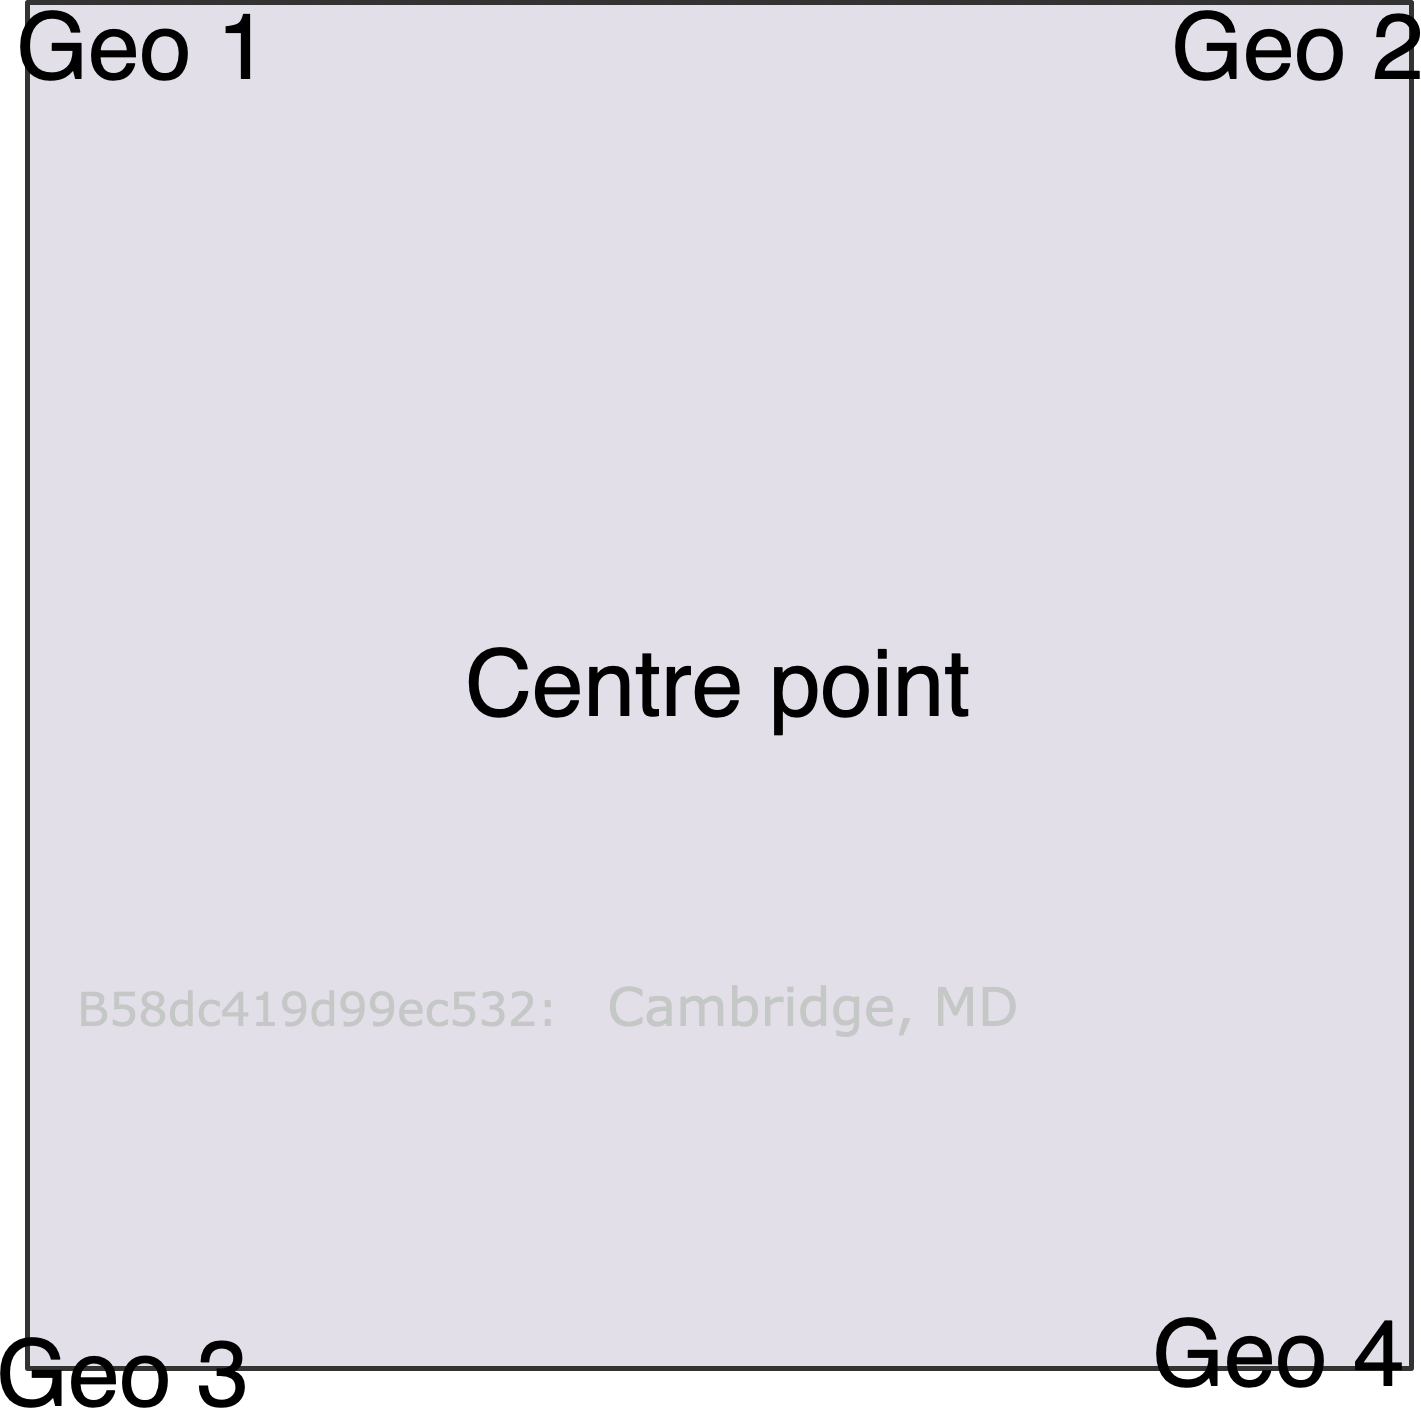
\includegraphics[width=.7\textwidth]{placeid.png}
    \caption{Illustration of Twitter place.id, a square defined by four geocode points, corresponding to a given place.}
    \label{fig:placeid}
\end{figure}

The place to which the ID is assigned is derived by Twitter through a process of \textit{data enrichment} using a combination of fuzzy matching of user entered location and GPS coordinates.

\subsection{Twitter atlas, first iteration}
\largerpage
It is possible to generate a useful atlas of tweets using the place.id alone, and indeed, the first iteration of the current atlas used this data. Here, the counts for each variant (\textit{ain't}+inf and \textit{didn't}+inf for each place.id were represented as pie charts on an interactive atlas. Pie charts were placed at the center point of the place.id area (see \figref{fig:placeid}). This was done using the \textit{leafletminicharts} package for R \citep{bachelier2021}. Using this package it was also possible to add a level of interactivity where the user can click on a pie chart and see a breakdown of the exact counts for that location. The user can then click on a variable and see a sample of the actual data from that place.

This was a valuable tool at this stage in the research process, allowing us to investigate different places, and offering a different way to probe the dataset by place. \figref{fig:aint_placeid} shows a screenshot of the interactive atlas focussing on the East North Central region of the US, specifically on the Chicago area.\largerpage

\begin{figure}
    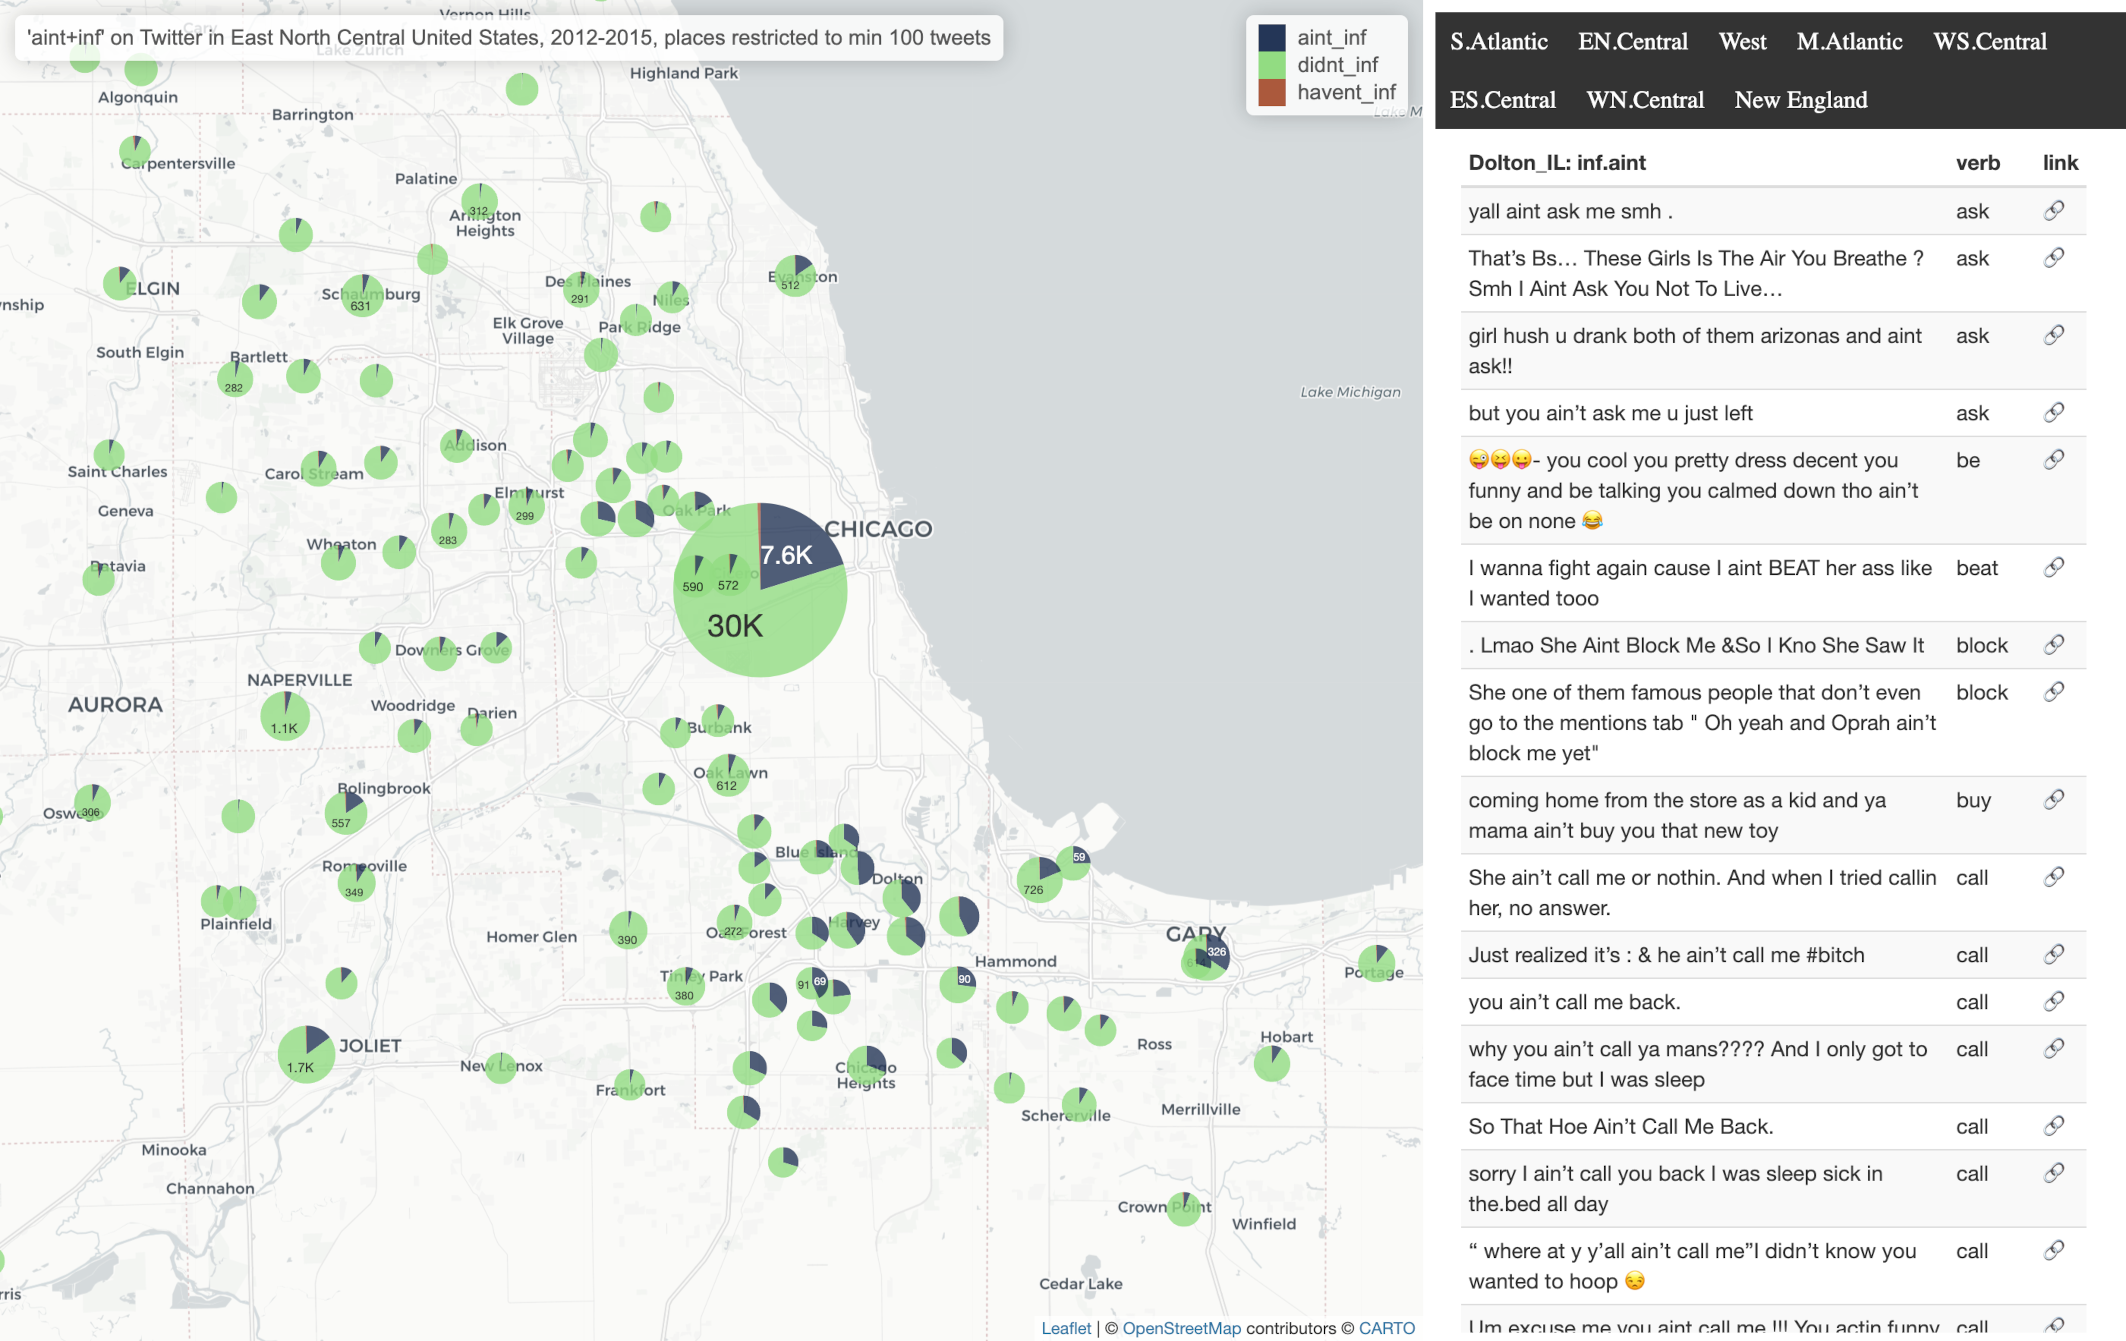
\includegraphics[width=\textwidth]{aint_placeid.png}
    \caption{Screenshot of the first iteration of the interactive atlas that uses Twitter place.ids rather than GPS points. Focus here is on the Chicago area. Interactive version available at \url{http://nwdialectatlas.uk/infaint/}.}
    \label{fig:aint_placeid}
\end{figure}


In order to be represented on the map, it was set that a place.id would have to have at least 100 tweets associated with it. This was done to ensure that enough data was present to draw statistically significant conclusions. In addition, this reduced the number of pie charts that had to be rendered on the map, improving legibility and performance (setting to lower that 100 per place meant that scrolling the atlas became too slow).{\interfootnotelinepenalty=10000\footnote{We should note here that the same limited dataset was used for the second iteration of the atlas, which was not necessary for that stage. We do not believe that this will affect the results for the second stage but future versions will have this legacy limit removed.}}

It became apparent immediately that there was geographic variation in the use of \textit{ain't}+inf versus \textit{didn't}+inf. Closer examination of places with high \textit{ain't}+inf use showed a pattern: all had high BAA populations. In \figref{fig:aint_placeid}, it is possible to see southern Chicago and Gary with high rates of \textit{ain't}+inf, represented in blue, both areas with high BAA populations, meanwhile northern and western areas have very low rates of \textit{ain't}+inf, which follows if \textit{ain't}+inf is distinctive to AAE.

\subsection{Twitter atlas, second iteration: linking to census data}
In order to show a systematic link between \textit{ain't}+inf use and BAA population, it is necessary to link Twitter place.id to demographic data. In the US, the most reliable demographic data is provided as part of the census. Census data is organised by tracts, with each defined by geographical polygons, stored as shapefiles. Each tract is associated with demographic information, such as race, about that geographic location. Tracts are defined for the purpose of administering the census, sometimes following political boundaries. They are the smallest geographic areas that are recorded with associated metadata.

However, it is not possible to directly link the Twitter place.id areas to tracts. Sometimes a place.id will encompass numerous tracts and other times, a census tract will contain several place.ids.

So, for the purposes of the present investigation, where the aim is to measure \textit{ain't}+inf against demographic data, it is necessary to have Twitter location data that is compatible with the location information provided for the US census. Associating tweets with census tracts was done using the point-in-polygon technique  (similar to \citealt{BlodgettGreenO’Connor2016}). This technique, illustrated in \figref{fig:pinp} is a method for calculating whether a given point falls within the bounds of a polygonal shape. In \figref{fig:pinp}, the red points have been found to be within the polygon.

\begin{figure}
    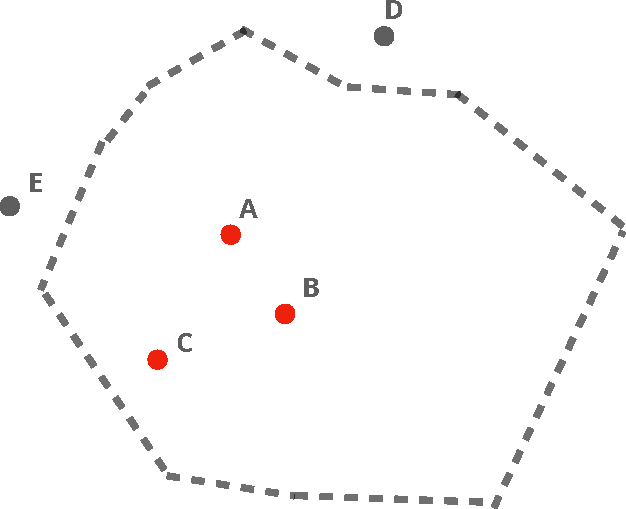
\includegraphics[width=0.5\textwidth]{image20.pdf}
    \caption{Illustration of point-in-polygon technique. Source: \url{https://datawanderings.com/2018/09/01/r-point-in-polygon-a-mathematical-cookie-cutter/}}
    \label{fig:pinp}
\end{figure}

The PinP technique was used to plot from which census tract a given tweet was sent. As we already know the racial demographic data for each tract, then the relative frequency of \textit{didn't}+inf and \textit{ain't}+inf  (\textit{ain't+inf index}) could be measured against the relative population of BAA against the total population (\textit{BAA index}).

\subsection{Retrieving census data}
US census data is freely available from census.gov and accessible directly in R using the \textit{tidycensus} package \citep{walker2023}. Tidycensus makes it straightforward to retrieve US Census data that is prepared for use with other R packages in the \textit{tidyverse} suite \citep{wickham2019}. It also makes it relatively easy to work with shapefiles using the sf package. A shapefile is a standard format for storing geographic data as vectors, in terms of points, lines, and polygons.  For our purposes, it is possible to use tract data to calculate an index of the BAA population by dividing BAA population by the total population for each tract. 

The index, hereafter referred to as the \textit{BAA index}, is calculated by dividing the BAA population by the total population. 

\[ \text{BAA index} = \frac{\text{BAA population}}{\text{total population}} \]

This can be seen in the map presented in \figref{fig:cook_county}.\footnote{An interactive version of the maps presented in this chapter is available at: \url{http://nwdialectatlas.uk/infaint/}.}


\begin{figure} 
    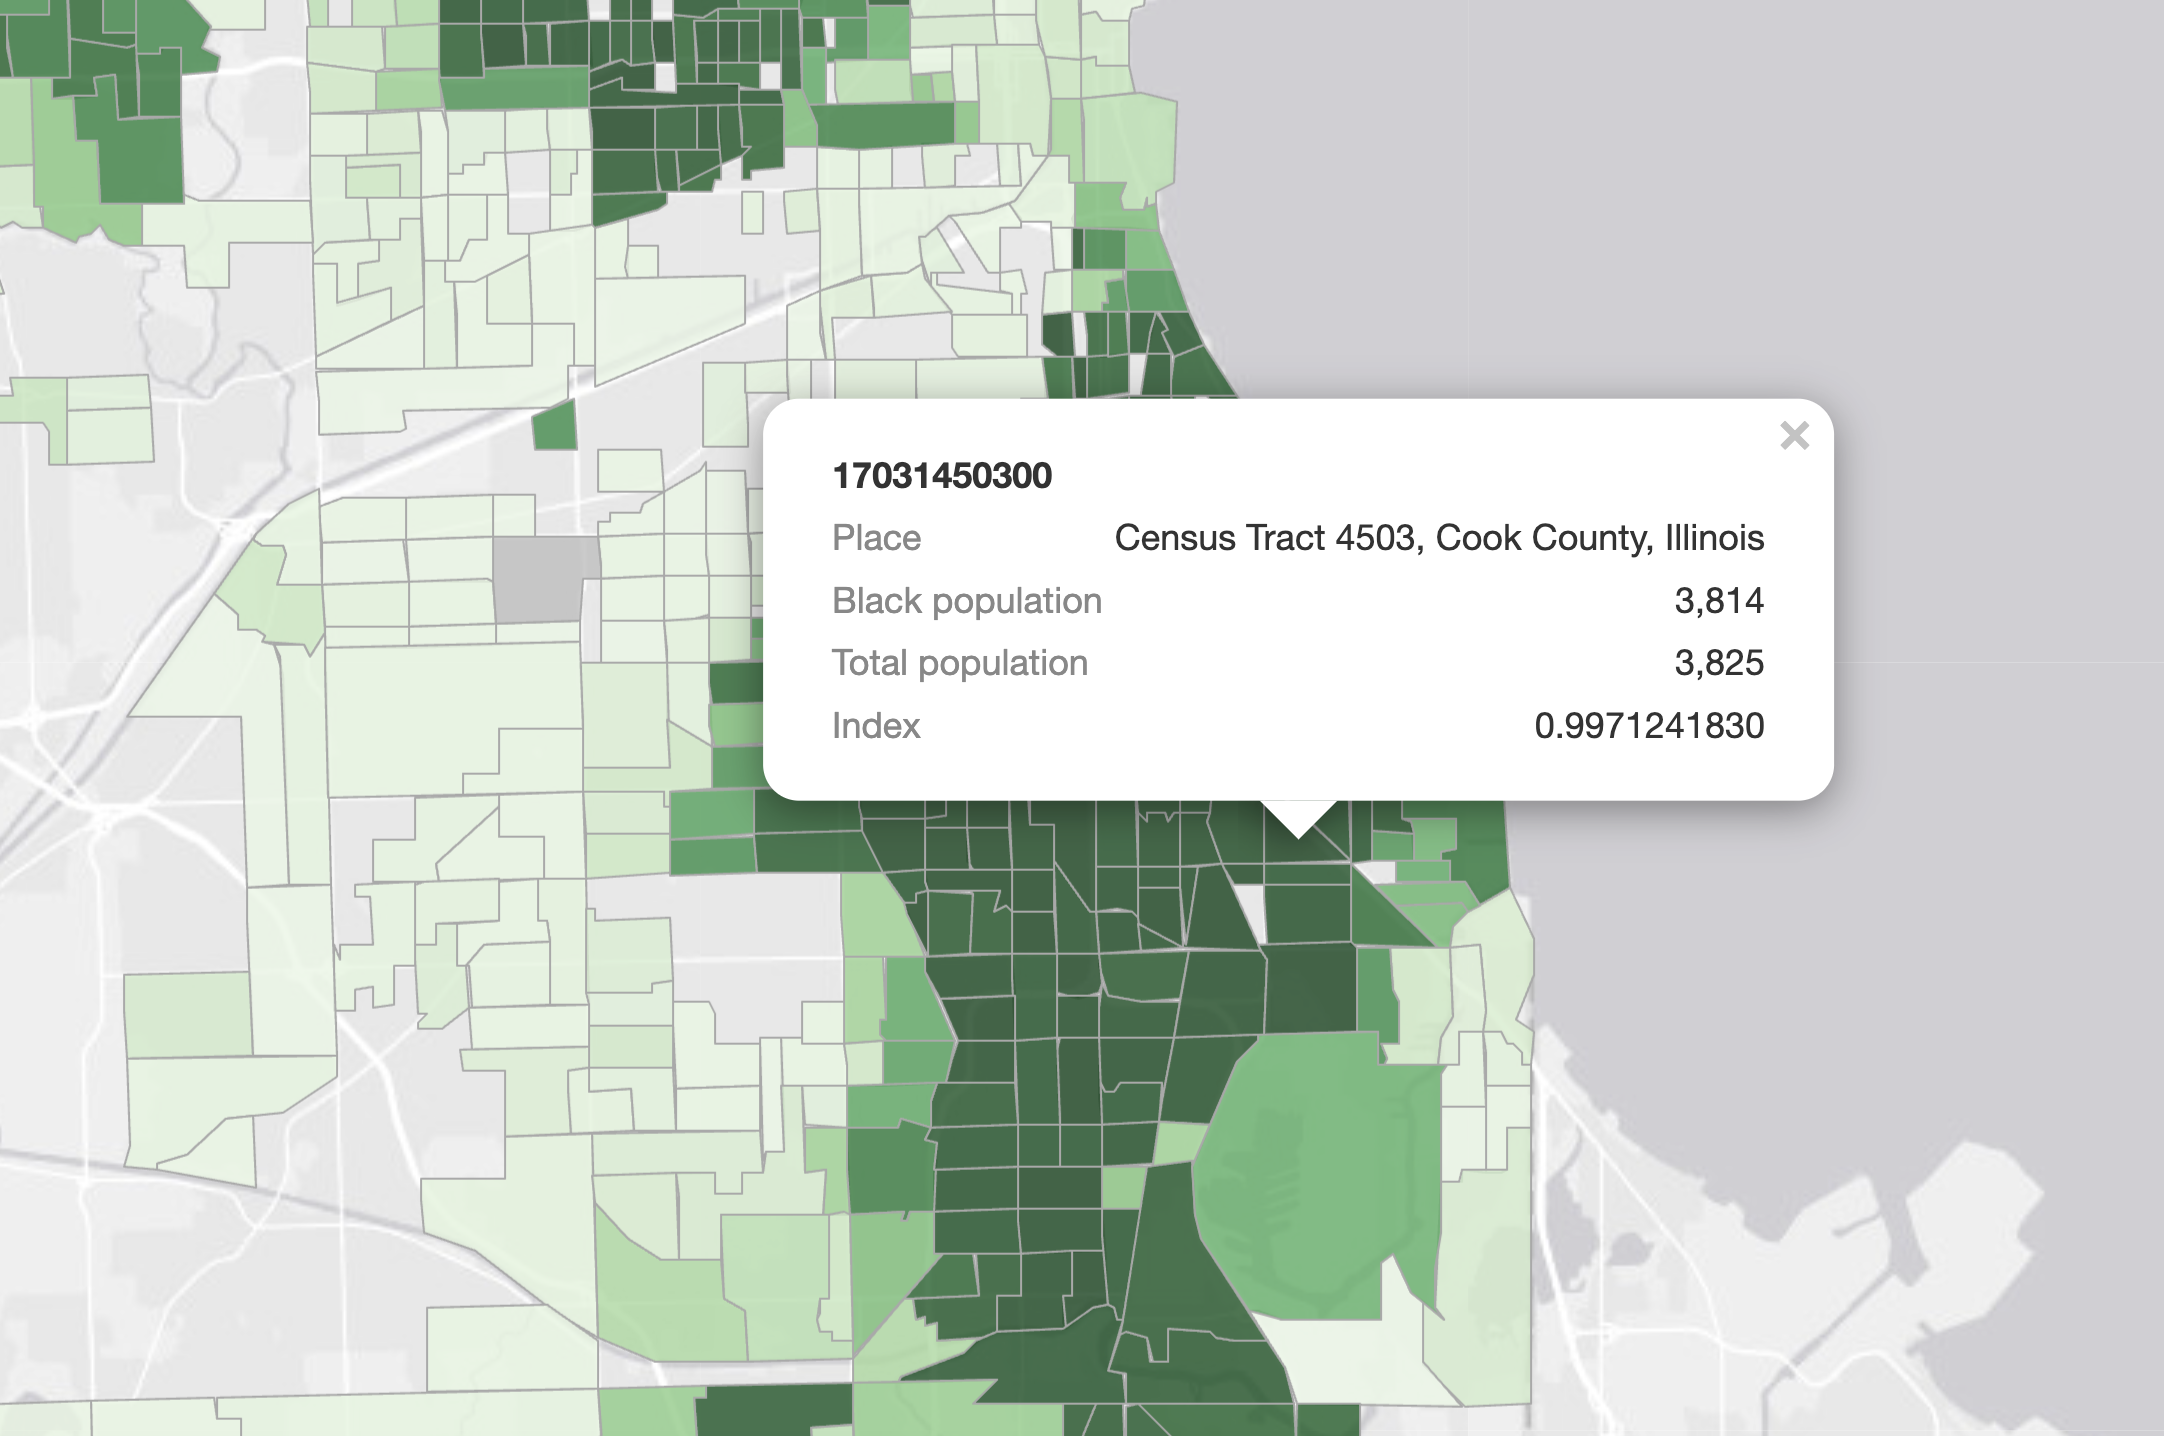
\includegraphics[width=\textwidth]{image7.png}
    \caption{\label{fig:cook_county}Cook County Census Tracts Tracts, based on data from US Census \textit{American Community Survey} 2011--2015 \citep{bureau2015}}
   
\end{figure}

\figref{fig:cook_county} is a map of Chicago, Illinois. The maps are divided into census tracts, each of which are linked to demographic information taken from the United States Census. The text-box in the center of the map displays information for one of the census tracts within the city: Cook County. This text-box appears as a pop-up when a census tract is clicked by the user.

In the case of Cook County, nearly 99.7\% of residents within this census tract are identified as BAA, which is reflected in the darker shade of green in this and surrounding census tracts.  Tracts with low populations of BAA people are represented by lighter shades of green.

\subsection{Mapping and plotting Twitter data with census data}
First, using the \textit{ain't+inf index} and \textit{BAA index} for each tract, two maps of the US were produced -- an \textit{ain’t}-usage-census-tract-map, and a racial-demographic-census-tract-map -- which could be used for a visual side-by-side comparison. If \textit{ain't}+inf is associated with BAA population groups, then we expect to see a visual similarity in the resulting maps.

Second, scatterplots were produced for each State, plotting \textit{ain't+inf index} against \textit{BAA index} with each point representing a single census tract.  If \textit{ain't}+inf is associated with BAA populations, then we expect to see a clear linear correlation between the two indices.

Finally, the data were broken down into high \textit{BAA index} (>90\%) and low \textit{BAA index} (<10\%) corresponding to high and low \textit{BAA index}. Boxplots could then be produced for each group, with each State represented by one box. Again, if \textit{ain't}+inf is unique to AAE, then we expect to see tracts with a high \textit{BAA index} coalescing (represented by short boxes) at a high rate of \textit{ain't}+inf and, conversely low \textit{BAA index} with low \textit{ain't}+inf.

\section{Results}
Here we present data on the three states under investigation: Illinois, Georgia and California. For each state, we start with heatmaps for Chicago, Atlanta, and Los Angeles and then present scatterplots for each respective state.  

We then present a comparison between \textit{ain't}+inf use across 13 states between high BAA population (>90\%) and low BAA population (<10\%).

\subsection{Illinois}
The two first maps, presented in \figref{fig:chigago}, compare BAA distribution (left) and \textit{ain't}+inf distribution (right). 

\begin{figure}
    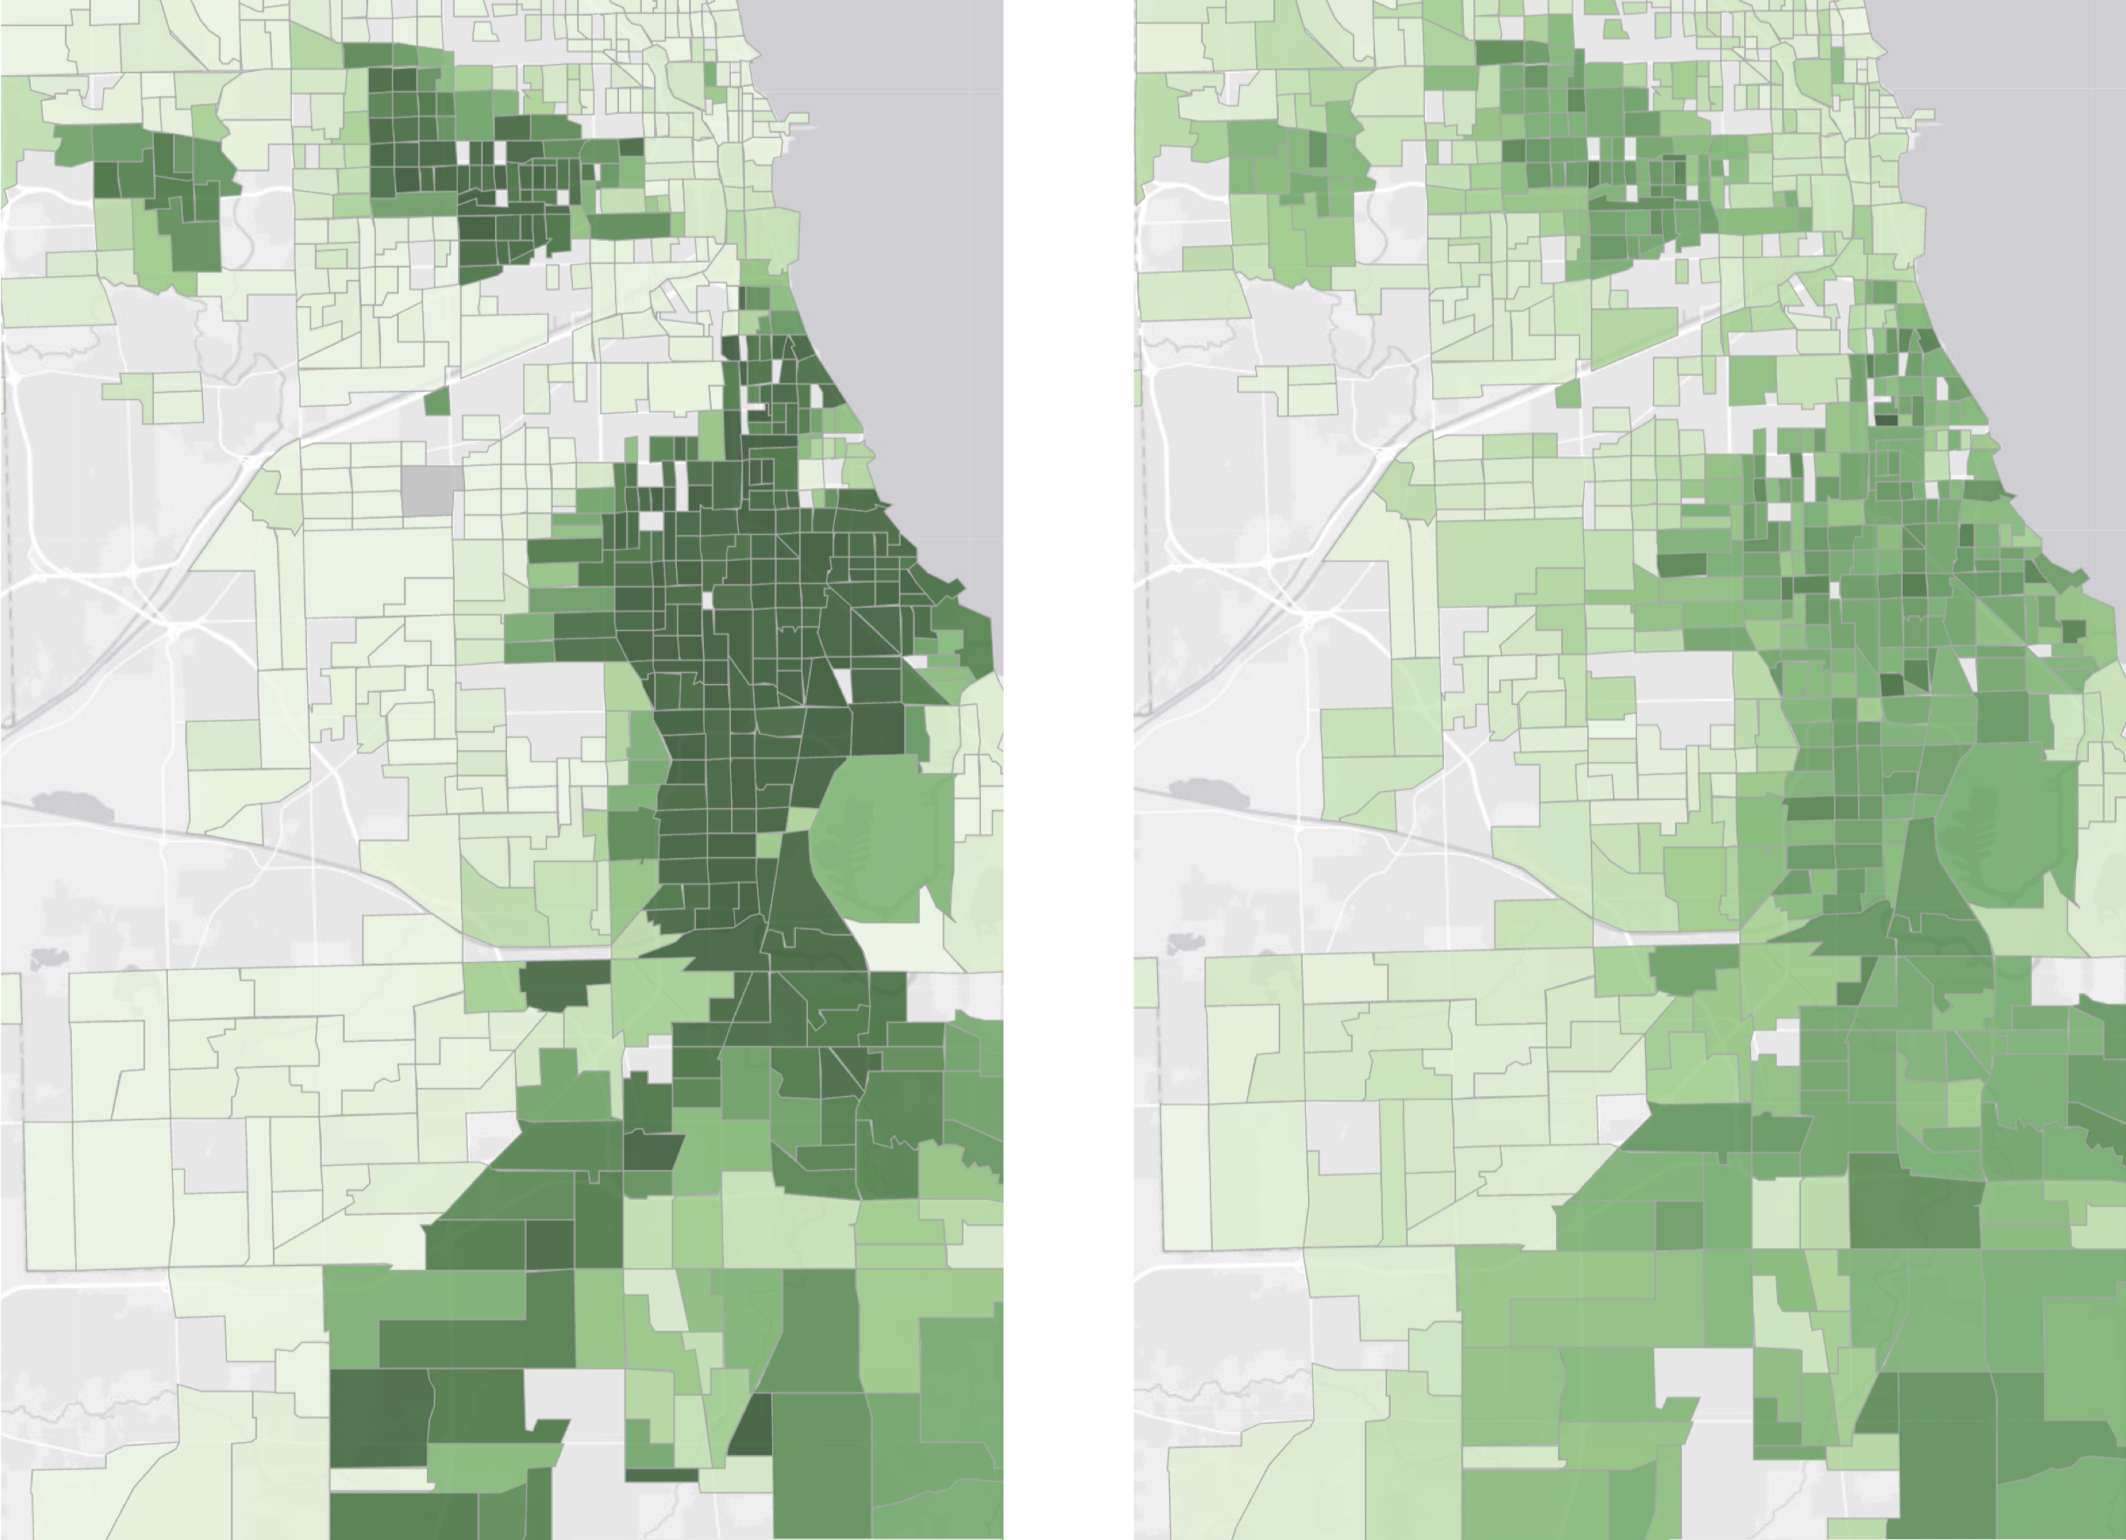
\includegraphics[width=\textwidth]{chicago.png}
    \caption{Chicago maps. Left = BAA Population Index, based on data from US Census \textit{American Community Survey} 2011--2015 \citep{bureau2015}; Right = \textit{ain't+inf index}}
    \label{fig:chigago}
\end{figure}

As stated, the distribution is represented by the \textit{BAA index}, which is calculated by dividing the BAA population of a given census tract by the total population of that census tract. 

From a simple observation of the two maps, it is evident that the prediction that \textit{ain't}+inf is associated with BAA population is borne out. The most concentrated areas of the \textit{ain't}+inf map are also the most concentrated areas of the \textit{BAA index} map. 

This is further clarified in the scatterplot for Illinois, in \figref{fig:illinois} which shows a clear correlation between \textit{BAA index} and \textit{ain't+inf index}; the higher the BAA population, the higher the \textit{ain't+inf index}.  The lower the BAA population, the lower the \textit{ain't+inf index}. 

\begin{figure}
    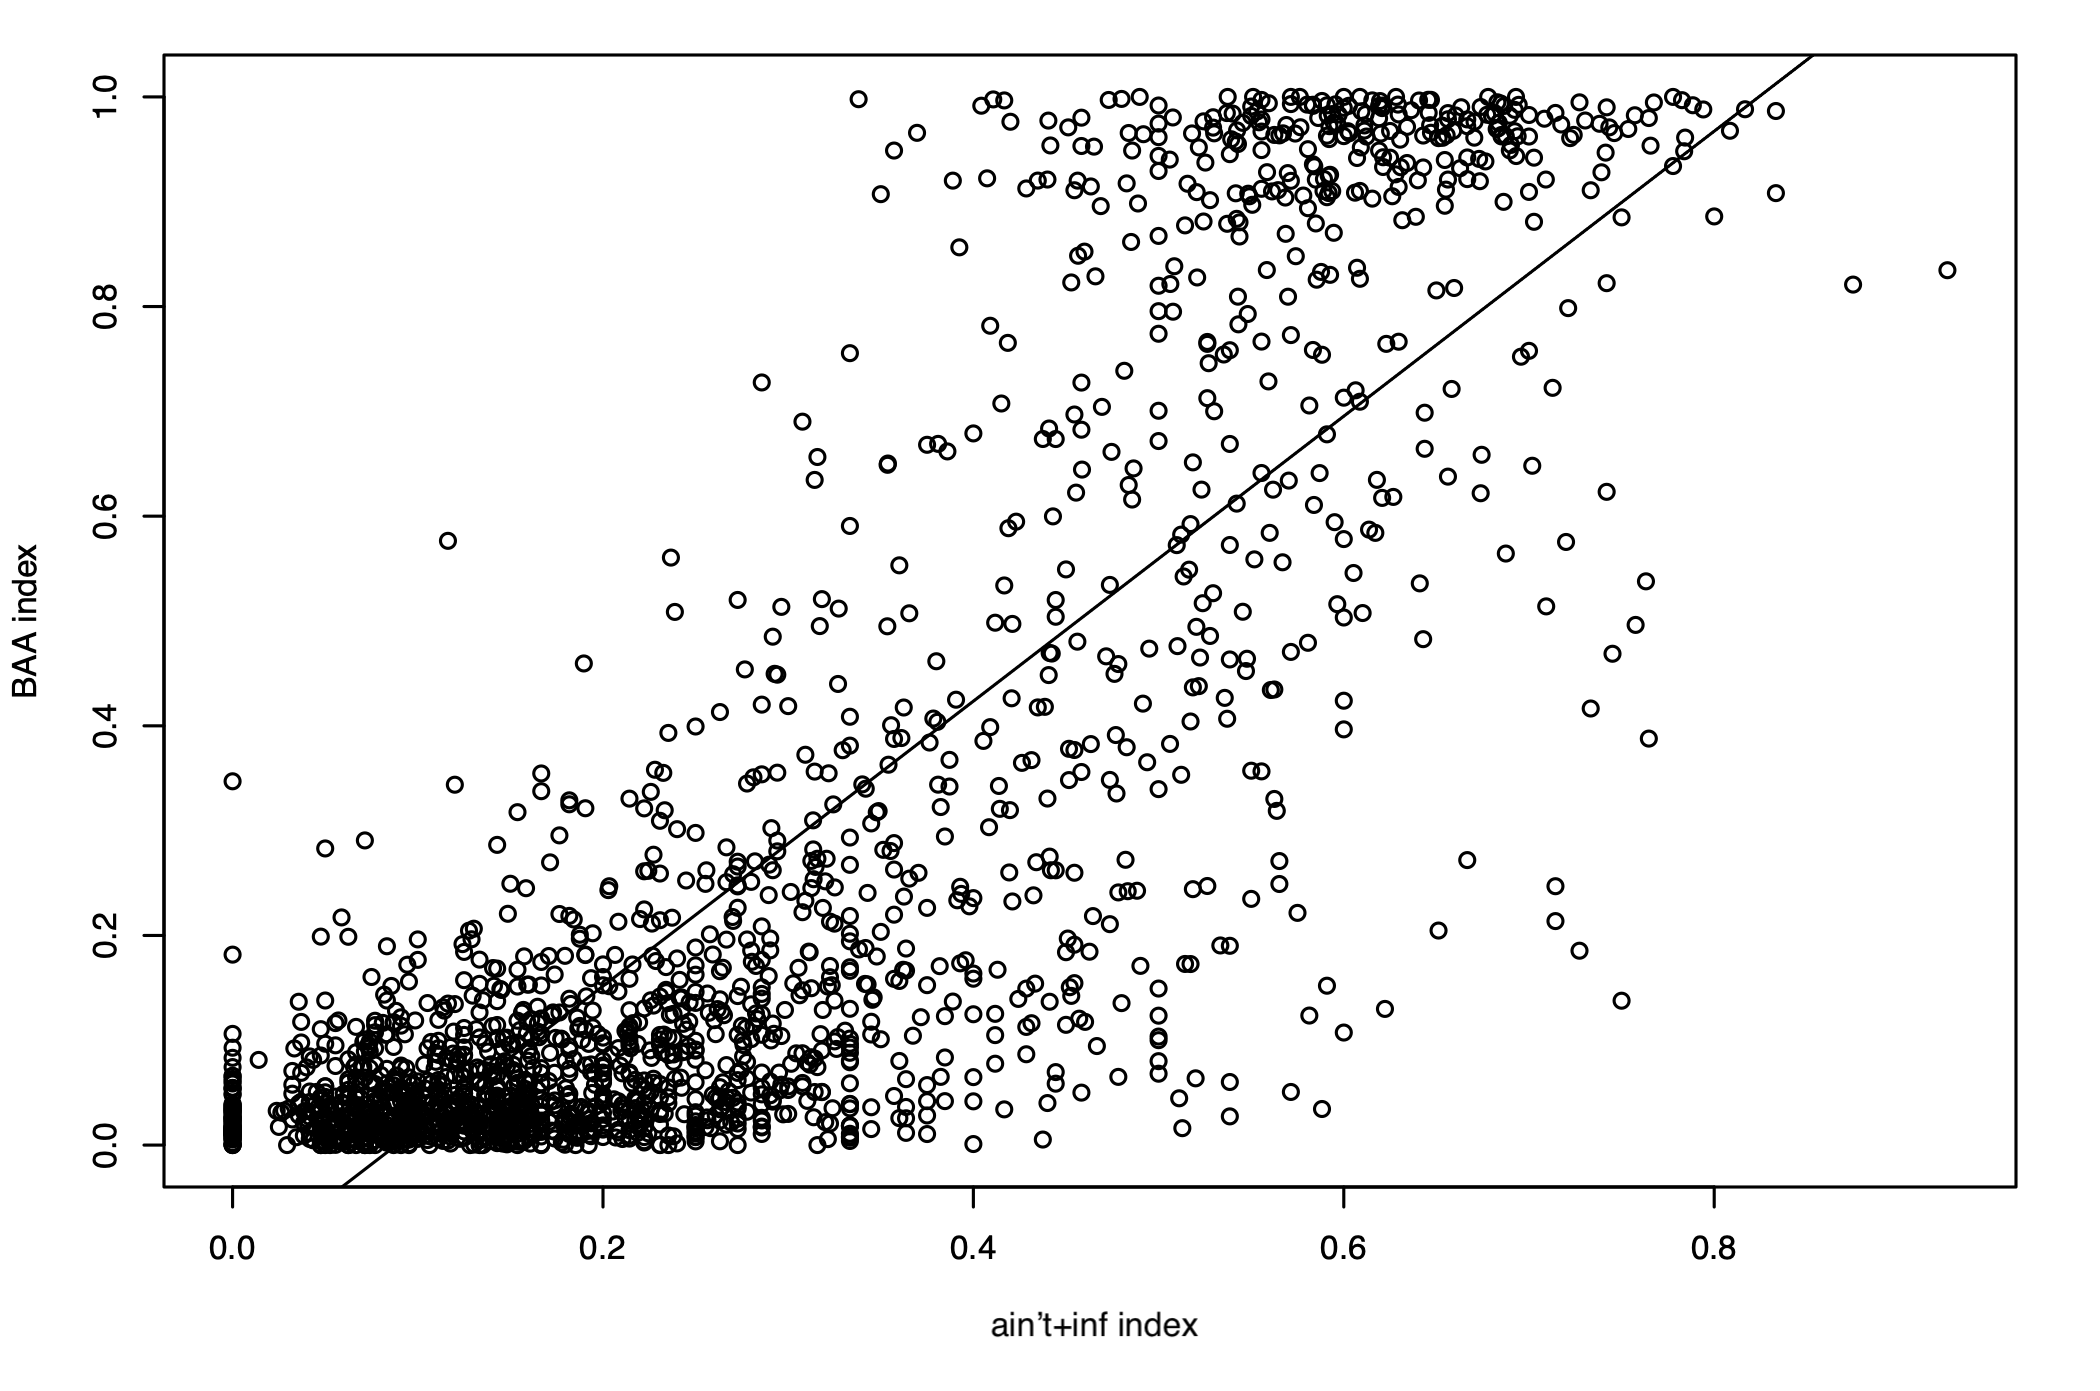
\includegraphics[width=\textwidth]{illinois.png}
    \caption{Scatter plot for Illinois: Vertical = BAA Population index; Horizontal = \textit{ain't+inf index}}
    \label{fig:illinois}
\end{figure}

Additionally, the segregation that exists in this part of the country is apparent, with large clusters of census tracts clustering at the top and bottom of the chart corresponding to tracts with nearly 100\% of residents identifying as BAA, or nearly 0\% BAA, while points in the center of the plot are more sparse, corresponding to there being far fewer tracts with a mixed population.

\subsection{Georgia}
The maps for Atlanta (\figref{fig:atlanta}) again show a clear similarity in distribution, comparing \textit{ain't}+inf and BAA populations.

\begin{figure}
    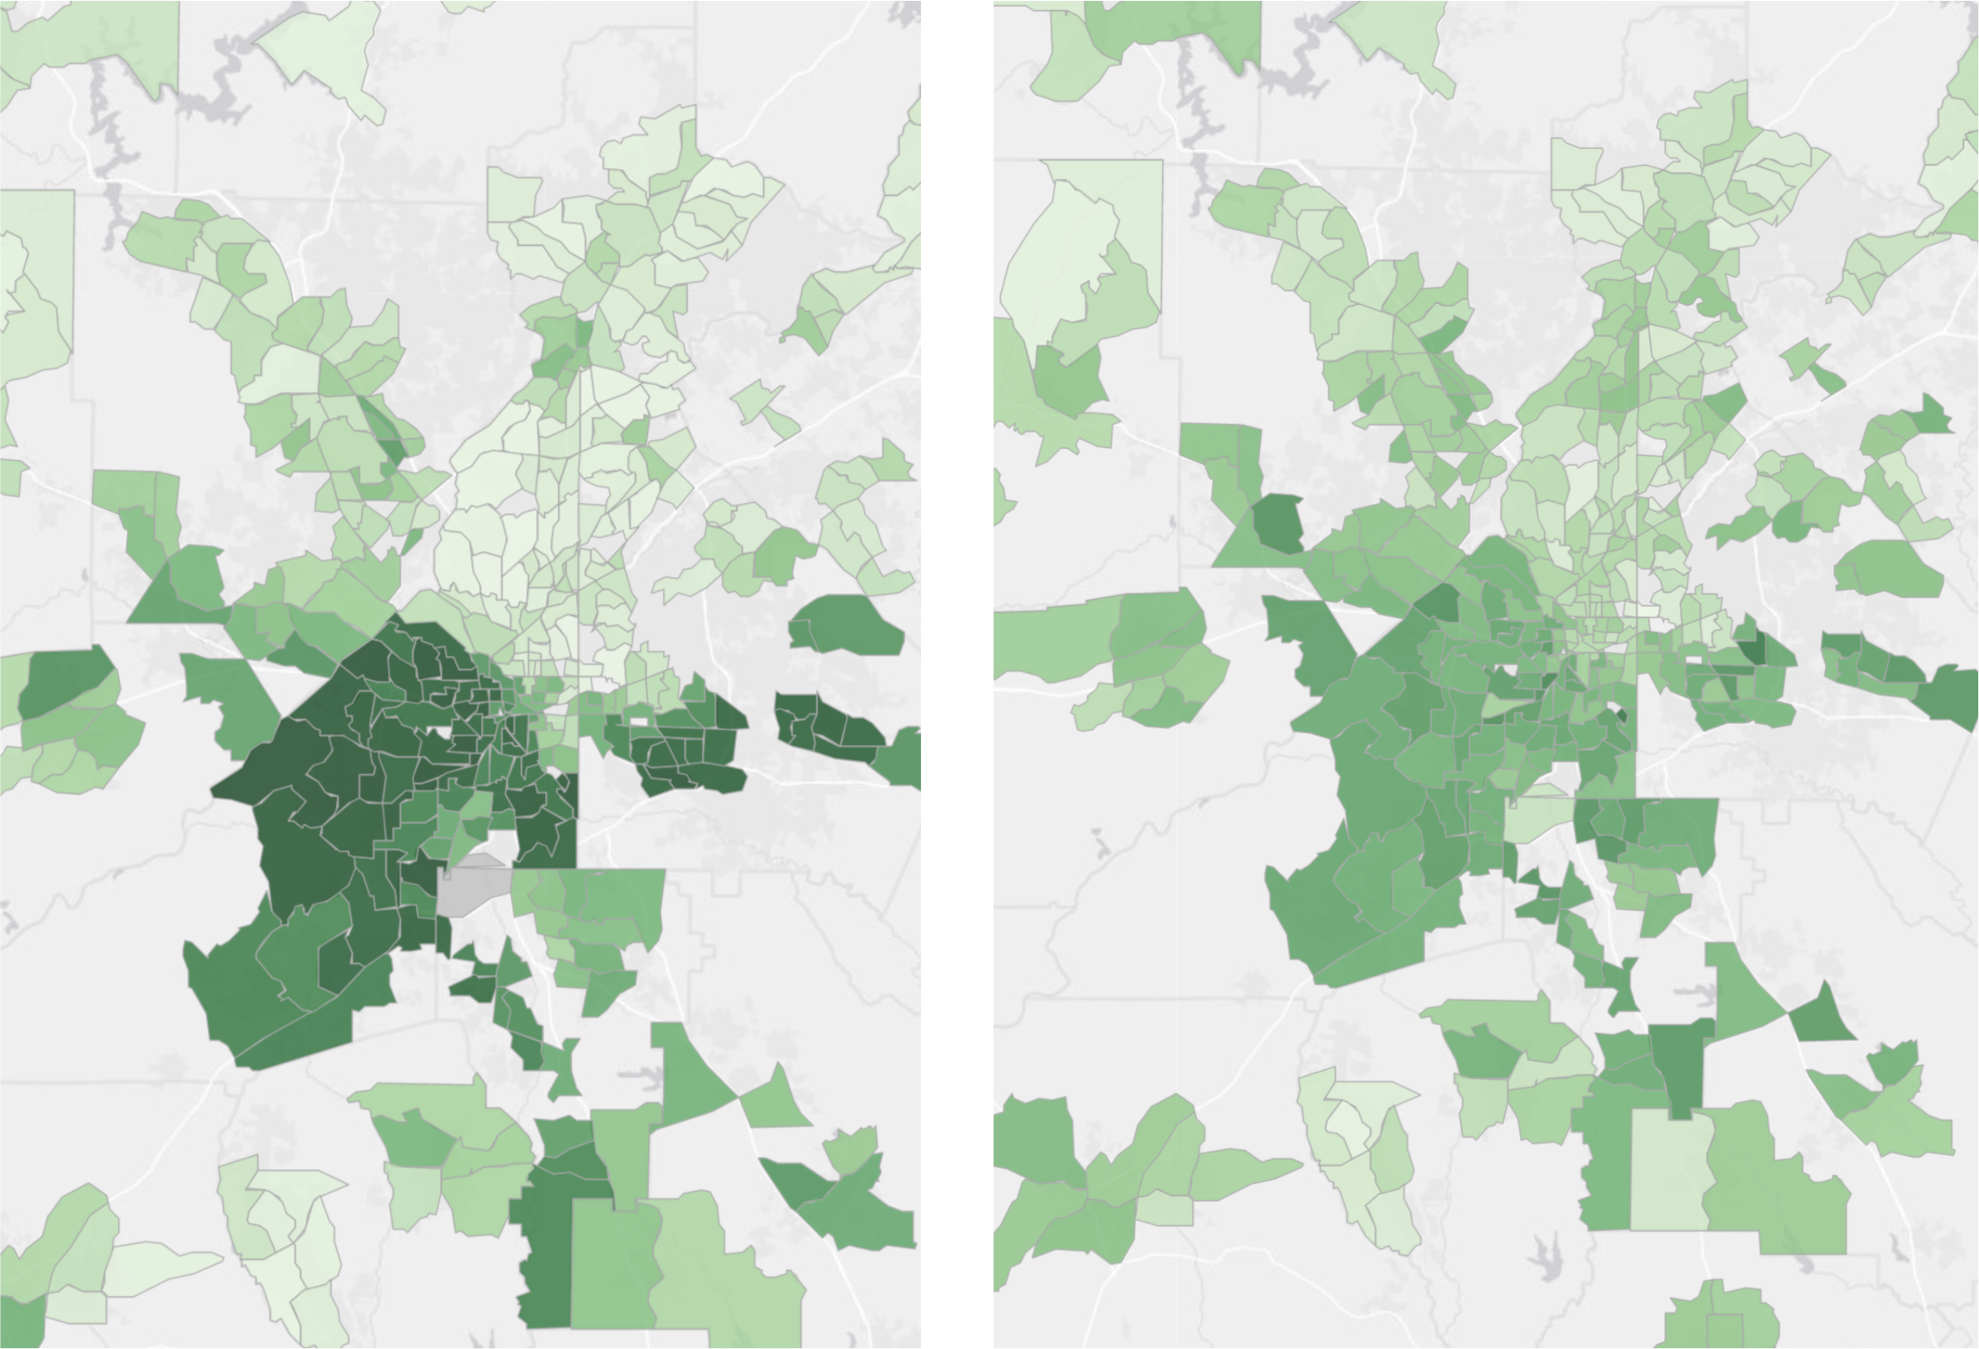
\includegraphics[height=.4\textheight]{atlanta.png}
    \caption{Atlanta maps. Left = BAA Population Index, based on data from US Census \textit{American Community Survey} 2011--2015 \citep{bureau2015}; Right = \textit{ain't+inf index}}
    \label{fig:atlanta}
\end{figure}

Meanwhile, the scatterplots for Georgia (\figref{fig:georgia}) contrast with those for Illinois (above) showing a smoother distribution of BAA population, while -- crucially -- still showing a clear correlation between \textit{BAA index} and \textit{ain't+inf index}.

\begin{figure}
    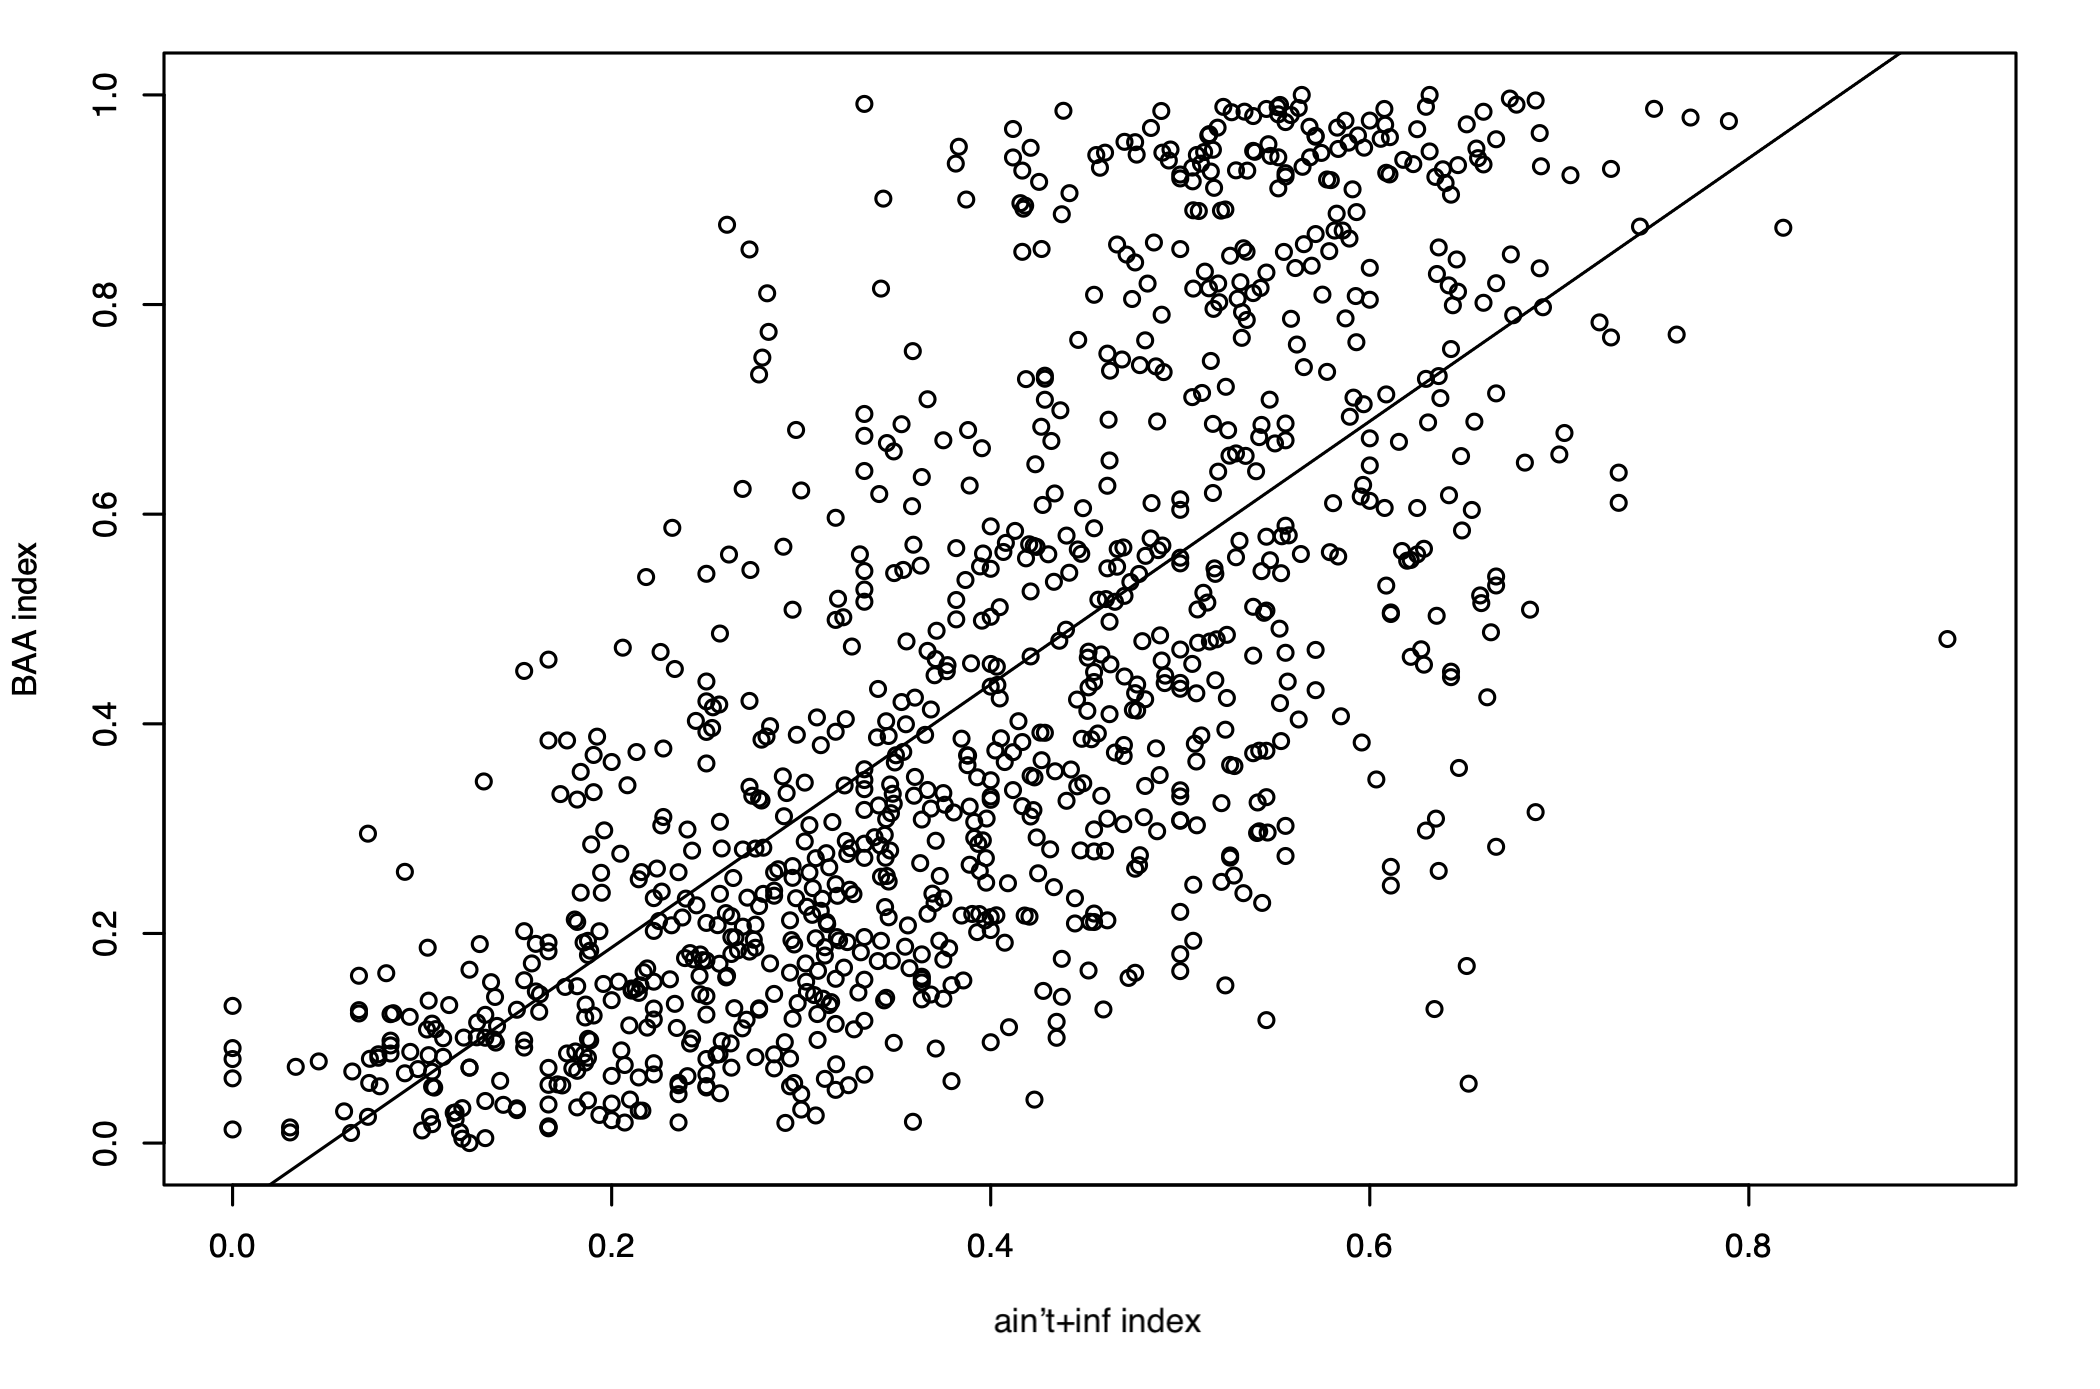
\includegraphics[height=.4\textheight]{georgia.png}
    \caption{Scatter plot for Georgia: Vertical = BAA Population index; Horizontal = \textit{ain't+inf index}}
    \label{fig:georgia}
\end{figure}

\subsection{California}
Particularly notable, however, is the absence of this correlation in the maps for Los Angeles, California (\figref{fig:losangeles}). While Illinois and Georgia show a very clear correlation between census tracts with high BAA populations and high \textit{ain't}+inf indices, results show that use of \textit{ain't}+inf in California is not only markedly lower, but less concentrated.

\begin{figure}
    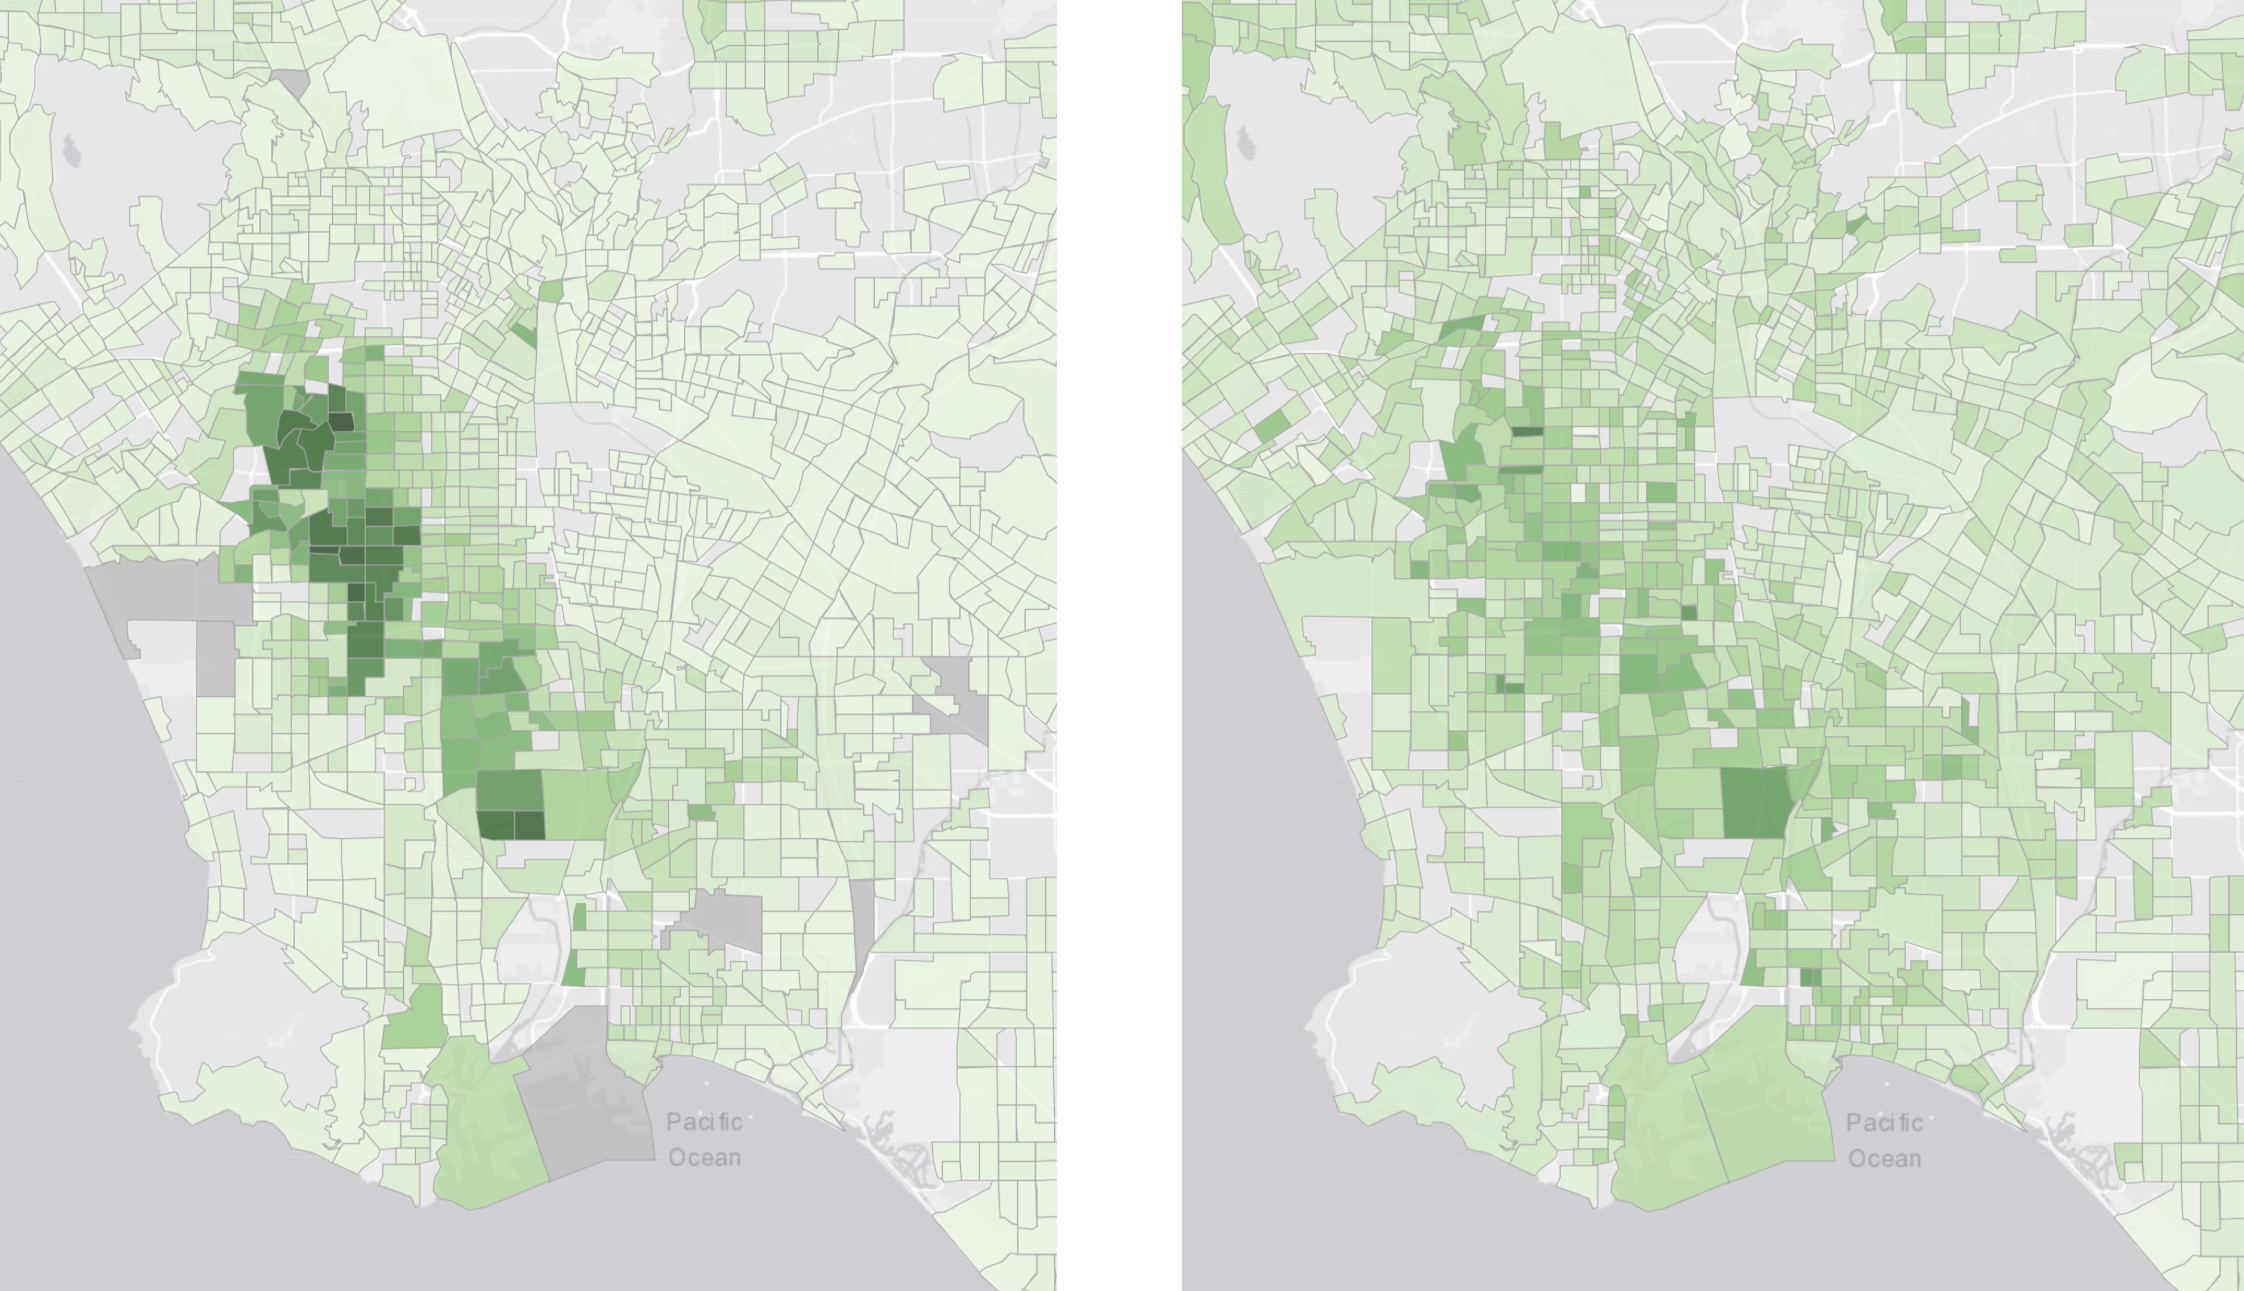
\includegraphics[height=.39\textheight]{losangeles.png}
    \caption{Los Angeles maps. Left = BAA Population Index, based on data from US Census \textit{American Community Survey} 2011--2015 \citep{bureau2015}; Right = \textit{ain't+inf index}}
    \label{fig:losangeles}
\end{figure}

The scatter plot in \figref{fig:california} supports this weaker correlation between \textit{BAA index} and the \textit{ain't+inf index} in California. Where the plots of the census tracts for Georgia and Illinois both show clusters of census tracts with a \textit{BAA index} of above 0.8, California shows a much lower number of census tracts which meet the same criteria.  

Of the tracts that do show a \textit{BAA index} of above 0.8, none show an \textit{ain't+inf index} above 0.4.  This is in contrast to Georgia and Illinois, where most tracts that show a \textit{BAA index} of 0.8 or above also show an \textit{ain't+inf index} of approximately 0.4 and above.


\begin{figure}
    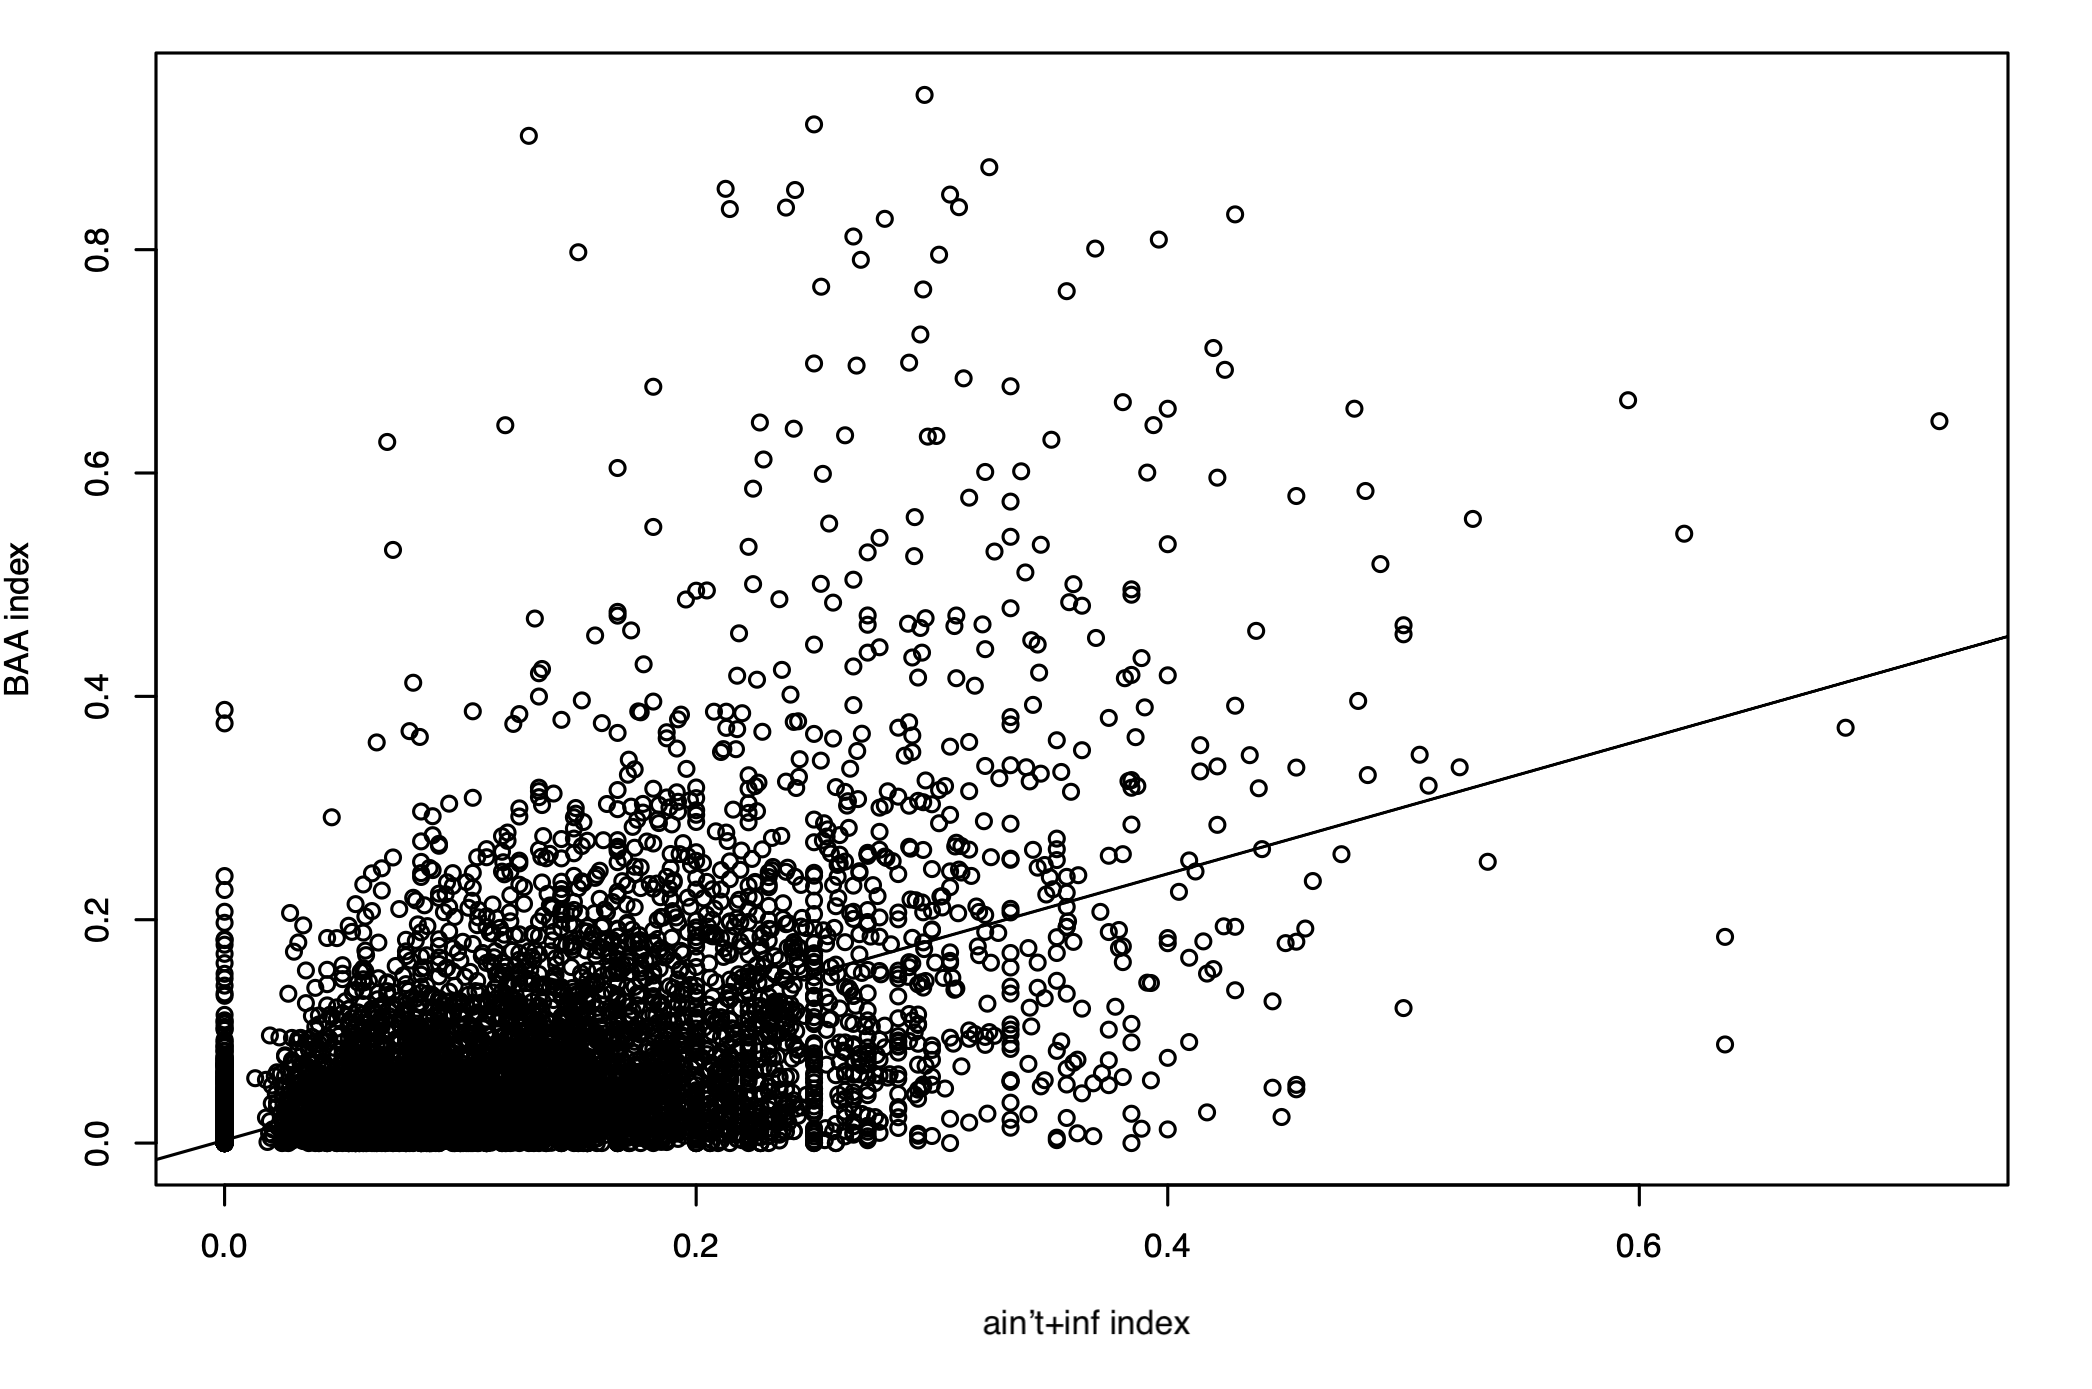
\includegraphics[height=.35\textheight]{california.png}
    \caption{Scatter plot for California: Vertical = BAA Population index; Horizontal = \textit{ain't+inf index}}
    \label{fig:california}
\end{figure}

\subsection{Comparing states}
Figures \ref{fig:states_10} and \ref{fig:states_90} are boxplots representing the \textit{ain't}+inf indices across 13 states in census tracts with 10\% or less BAA/BAA population and 90\% or more BAA/BAA population, respectively, and shows that unlike other states, the \textit{ain't+inf index} in California remains relatively low regardless of \textit{BAA index}.

The boxplots in Figures \ref{fig:states_10} and \ref{fig:states_90} further underscore the marked difference in \textit{ain't}+inf use in California, as compared to other states.  Both in census tracts with 0.9 \textit{BAA index} or greater and census tracts with 0.1 \textit{BAA index} or less, the average \textit{ain't+inf index} remains relatively low, and does not increase regardless of racial population density.  Also notable are \textit{ain't}+inf rates in Alabama (AL), Louisiana (LA), and South Carolina (SC), which all show slightly higher \textit{ain't}+inf indices among census tracts with 0.1 \textit{BAA index}, showing at around 25\% usage where other states show >20\% usage.

\vfill
\begin{figure}[H]
    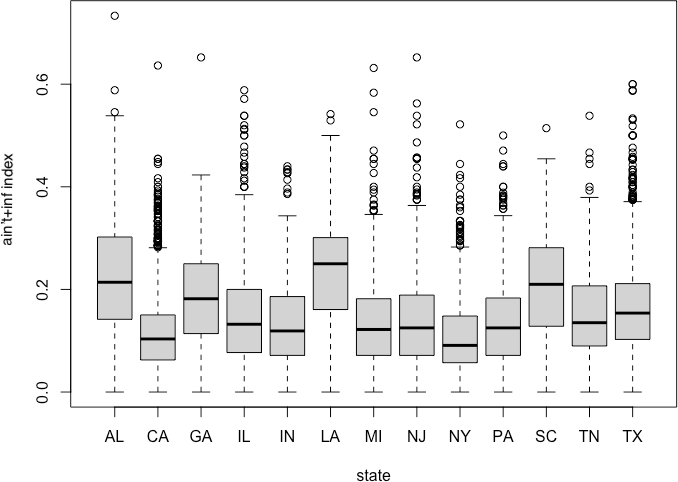
\includegraphics[height=.4\textheight]{states_10.png}
    \caption{Boxplot showing \textit{ain't+inf index} for tracts with <10\% BAA population}
    \label{fig:states_10}
\end{figure}
\vfill
\pagebreak

\begin{figure}[t]
    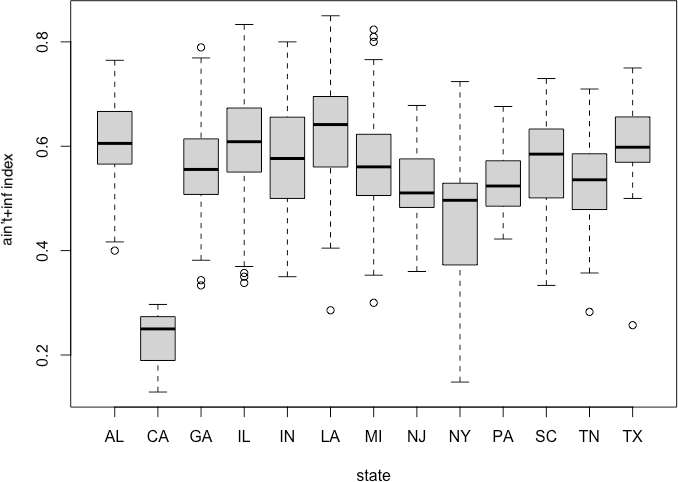
\includegraphics[height=.4\textheight]{states_90.png}
    \caption{Boxplot showing \textit{ain't+inf index} for tracts with >90\% BAA population}
    \label{fig:states_90}
\end{figure}


\section{Analysis}
The results above confirm the conclusions reached in previous research, which found a correlation between the use of \textit{ain’t-for-didn’t} constructions and BAA speakers. As a result, they also support previous findings \citep{eisenstein2013,jones2015,willis2020} that language use on social media platforms such as Twitter patterns with natural language distributions found using traditional methods.

\textit{Ain't}+inf is considered to have been originally relatively rare in early AAE in the Southern US, with the structure having been innovated in the northern cities after the Great Migration. If this is indeed the case, the current distribution shows a continued and near-complete spread of \textit{ain't}+inf within BAA communities in the United States from the northern urban centers to southern urban centers. 

This is important to note when we consider \citet{fisher2022}, whose analysis suggested that \textit{ain't}+inf and other forms of \textit{ain't-for-didn’t} were used more frequently among speakers who were born and raised in Philadelphia than they were among speakers who had recently migrated from the South. The data also reveal that this spread has not reached as far as California, where \textit{ain't}+inf is shown to be relatively infrequent, and uncorrelated with the distribution of BAA populations.

Why this North-South spread has occurred, and why it has not spread west to California is unclear at this stage, but is a topic ripe for future investigation. A first point of investigation here would be to analyse migration patterns from the northern cities to the south. Cities such as Atlanta have re-emerged in recent years as BAA cultural centers, attracting new waves of BAA migrations. It may also be partly explained by ongoing family and social ties between the north and south that have facilitated the spread of \textit{ain't}+inf south, but not west. It will be interesting to see if \textit{ain't}+inf is part-way through a process of diffusion, and will eventually reach California, or if it will remain a difference between the varieties of AAE in west and east.


\section{Conclusion}
This paper discussed variationist studies in African-American English and aimed to contribute to the study of syntactic variation therein by conducting a study of language data mined from Twitter via the Twitter API. 

We presented an analysis which also used Twitter data to confirm analyses reached by more traditional methods in previous literature, thus showing the viability of Twitter data in the study of syntactic variation in AAE.  To collect the data, we examined the parameters through which infinitival \textit{ain't} occurred and isolated it from other uses of \textit{ain't} which were more ambiguous.  

To map the data, we calculated an index of infinitival \textit{ain't} use and used a point-in-polygon approach to map the geospatial metadata within each tweet within census tracts taken from the US Census. The resulting maps show a correlation between infinitival \textit{ain't} and census tracts with high BAA/African-American populations in Georgia and Illinois, but show a much weaker correlation, as well as a much lower average \textit{ain't+inf index} in California.  Data shows that this weaker correlation holds regardless of race.

The results of each map were confirmed by scatter plots and box plots which also showed a correlation between \textit{BAA index} and \textit{ain't+inf index} in communities with high populations of BAA/African-American identifying residents, according to the US Census, with the exception of California.

These results indicate a likely difference in both the frequency and manner of \textit{ain't} usage in the United States, despite previous descriptions of the variety as uniform within urban centers. These results represent a starting point for future researchers to analyse them in more detail via alternate methods such as surveys and/or interviews.

Finally, we have shown how the language-first approach adopted here using Twitter data is compatible with, and reflective of, already-established conclusions gleaned from more traditional identity-first analyses.

\section{Future directions}\label{sec.fut}
As stated at the outset, the work presented in this chapter represents the first step in what is planned to be a much larger atlas of AAE use using both Twitter data and data drawn from traditional methods. With this said, the most pressing next steps are:\largerpage[2]


\begin{enumerate}
    \sloppy
	\item Investigate the underlying causes for the apparent spread of \textit{ain't}+inf south from the northern cities to those in the south, while not to western coastal areas. Could this be explained by the maintenance of cultural ties (or lack thereof) and migration patterns?
    \item Investigate other forms of \textit{ain’t}: correlations between other forms of \textit{ain’t} and BAA Populations in order to check the hypothesis that Twitter data shows that \textit{ain't}+inf is uniquely tied to AAE.  For example, do other uses of \textit{ain’t}, particularly \textit{ain't+perfective} (as in \textit{ain't seen}), also show a high correlation with BAA communities?
    \item Investigate weak verbs: the extent to which weak verbs (\textit{move}, \textit{raise}), consonant cluster reduction ( etc.) and other phonological properties of AAE influence the orthographical spelling of verbs on Twitter, and could mean some of what appears to be \textit{ain't}+inf is actually perfective \textit{ain't}.
    \item Investigate contextual variation: the extent to which contextual variation exists in the use of \textit{ain't}+inf across different regions.
    \item Build the Atlas. Begin the process of compiling all of this into an interactive atlas. Combine different visualisation methods (such as pie charts in first map). Research and add other AAE parts of speech.
    \item Investigate alternative methods. Use alternative method for getting location data -- \textit{I grew up in} rather than GPS point from where a tweet was sent.
    \item Investigate outliers among box plots and scatter plots.  Identify the locations of outlier census tracts, in order to further investigate the context behind outlier tracts.  In the case of the boxplots, this context also addresses the outliers in the BAA minority group, and the disparity in the number of outliers in the BAA majority group.
\end{enumerate}

\section*{Abbreviations}
\begin{tabularx}{\textwidth}{@{}lQ@{}}
BAA  & {Black and African American} \\
inf  & {infinitive verb} \\
\end{tabularx}

\printbibliography[heading=subbibliography,notkeyword=this]
\end{document}
